\chapter{New efficient edge-based zonotope vertex enumeration}
\label{chapter:2}
\usection{Introduction}
To understand how \emph{in silico} isometric force feasible sets encompass both muscle tension interactions and muscle biomechanical characteristics, notably their paths along bones and their exertable tensions, this thesis delves into the geometric process of exerting maximal isometric forces. A force feasible set $\mathcal{F}$ is described by two successive geometric set-theoretic operations: 1) the projection of a tension feasible set $\mathcal{T}$ onto the joint torque space, creating the \emph{torque feasible set}, and 2) the intersection of the torque feasible set with a vector space. 

A main objective of this thesis is to understand the set-theoretic properties of force feasible sets to guide the personalization of muscle parameters in musculoskeletal models, which is addressed in Chapters \ref{chapter:4} and \ref{chapter:5}. As a first step toward this understanding, this chapter studies specifically the projection of the tension feasible sets — more precisely, it examines how the torque feasible set encompasses muscle properties. 

To assess how tension interactions are projected onto the torque space, different models of these interactions must be considered. Chapter \ref{chapter:1} explained that varying the model of the tension feasible set leads to distinct force feasible set characterizations, such as force polytopes and force ellipsoids. This chapter and Chapter \ref{chapter:3} are strongly linked, as they focus on tension feasible set modeling and its impact on the resulting geometric construction. While this chapter concentrates on polytopic representations, Chapter \ref{chapter:3} will study more rounded shapes. Both chapters require different mathematical frameworks to better account for tension feasible set modeling; hence, they are presented separately. 

With $\mathcal{T}$ modeled as an orthotope (a hyperrectangle), this chapter approaches the understanding of the projection process through a combinatorial lens. This approach, which encompasses mathematical results related to \emph{counting} objects, is particularly well-suited for polytope-related studies, as polytopes possess inherent combinatorial properties that reflect their shape and volume (\cite{grunbaumConvexPolytopes2013}). However, such properties can be challenging to discern, as they may not have an explicit form or simple interpretation. Dedicated algorithms can provide a different perspective on these results by iteratively examining combinatorial solutions to a problem and selecting specific ones. This selection process is inherently informative (\cite{barvinokComputingEhrhartQuasipolynomial2005}; \cite{lopezPolytopeIntersectionHalfspaces2024a}).

Therefore, this chapter presents an algorithm that computes the vertices delimiting the projection of a tension feasible set, modeled as a hyperrectangle, onto the torque space. The resulting shape is termed a \emph{zonotope} and is a specific type of polytope exhibiting central symmetry. Because these vertices are \emph{unique} to a zonotope, their enumeration reflects how the bounds of muscle tensions are projected onto the torque set. The following paragraphs focus on clearly introducing this concept in the context of \emph{in silico} force feasible sets.

In this thesis, $\mathcal{T}\subset \IR^m$ denotes the set of all exertable tensions by $m$ muscles, also termed the tension feasible set. The force feasible set $\mathcal{F}\subset \mathbb{R}^3$ at the end effector of an $n$ degrees-of-freedom kinematic chain in a given posture is expressed as:
\begin{align*}
    \mathcal{F} = \left\{\mathbf{f}\in\IR^3\mid \exists \mathbf{t}\in \mathcal{T},\quad J^T\mathbf{f} = -L^T\mathbf{t} - \mathbf{G}\right\}
\end{align*}
where $J^T\in \mathbb{R}^{n\times 3}$ is the projection of the end-effector Cartesian forces onto the torque space, $L^T\in \IRnm$ is the projection of muscle tensions onto the torque space, and $\mathbf{G}\in\IRn$ is the gravity torque vector.
As we will focus in this chapter on only the projection of $\mathcal{T}$ onto the torque space, we define the \emph{torque feasible set} as the following:
\begin{align*}
    \left\{\tau \in \IR^n \mid \exists \mathbf{t}\in\mathcal{T}, \quad \tau = -L^T\mathbf{t} - \mathbf{G}\right\}
\end{align*}

$\mathcal{T}$ is assumed to be shaped as a $m$-orthotope (a hyperrectangle in $m$ dimensions) (Fig. \ref{fig:tension_set_orthotope}). This shape models how muscles can act together: it allows all muscles to exert their maximal tension simultaneously, which will be necessarily reflected onto the torque space (Fig. \ref{fig:joint_torque_simple_2D}). More precisely, for each exertable tension $t_i$ of a muscle $m_i$, there exist positive lower and upper bounds, denoted $\underline{t_i}$ and $\overline{t_i}$, defining the feasible tensions exertable by muscle $m_i$. The upper bound corresponds to the feasible muscle tension when the muscle is fully activated, while the lower bound relates to its passive tension when it is not activated.
\begin{figure}[!htb]
%   \captionsetup{justification=centering}
  \begin{minipage}{0.39\linewidth}
    \centering
    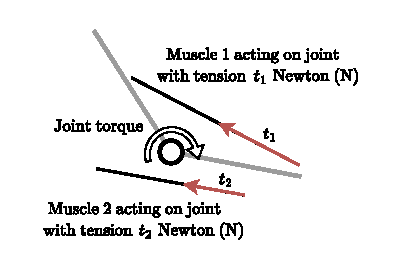
\includegraphics[trim={20 0 20 0}, clip, width=1\linewidth]{img/chapter_2/joint_torque_simple_2D.pdf}
    \caption{Simplified arm with one degree-of-freedom equipped with two muscles described as segments.}
    \label{fig:joint_torque_simple_2D}
  \end{minipage}
  \hfill
  \begin{minipage}{0.59\linewidth}
    \centering
    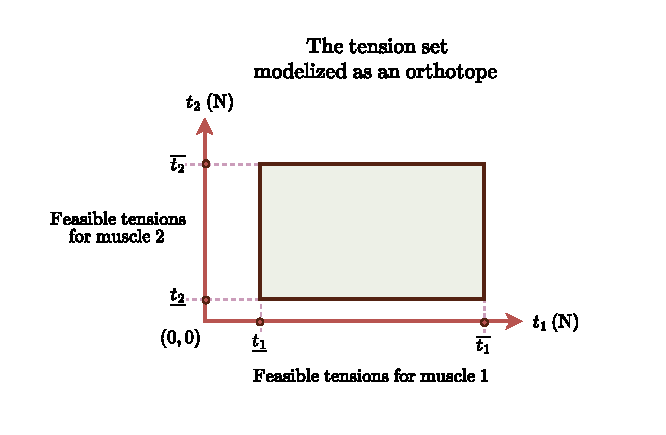
\includegraphics[trim={25 20 40 16}, clip, width=0.92\linewidth]{img/chapter_2/tension_set_orthotope.pdf}
    \caption{A muscle exerts tension in a feasible range of values. The set of all tension combinations $\mathcal{T}$ is shaped as an orthotope.}
    \label{fig:tension_set_orthotope}
  \end{minipage}
\end{figure}

While the assumption of independent exertion of tensions is plausible for a cable robot, human muscle activations are subject to neuromotor control, the laws of which are not yet fully understood. In cable robotics, if the feasible tensions of the cables (modeled as line segments) are assumed to be independent, the tension feasible set $\mathcal{T}$ takes the shape of an orthotope.

Geometrically, the torque feasible set is thus a \emph{zonotope}, \emph{i.e.}, a specific type of polytope described as a projection of a higher-dimensional cube. To compute the vertices of a zonotope, note that an $m$-orthotope is the image of an $m$-cube under an invertible affine transformation. Without loss of generality, $\mathcal{T}$ can be equated to the $m$-dimensional cube $[0,1]^m$, as shown in Figure \ref{fig:invertible_transfo_cube_orthotope}. An $m$-orthotope and an $m$-cube are said to be \emph{affinely equivalent}. 
\begin{figure}[!htb]
  \captionsetup{justification=centering}
  \begin{minipage}{1\linewidth}
    \centering
    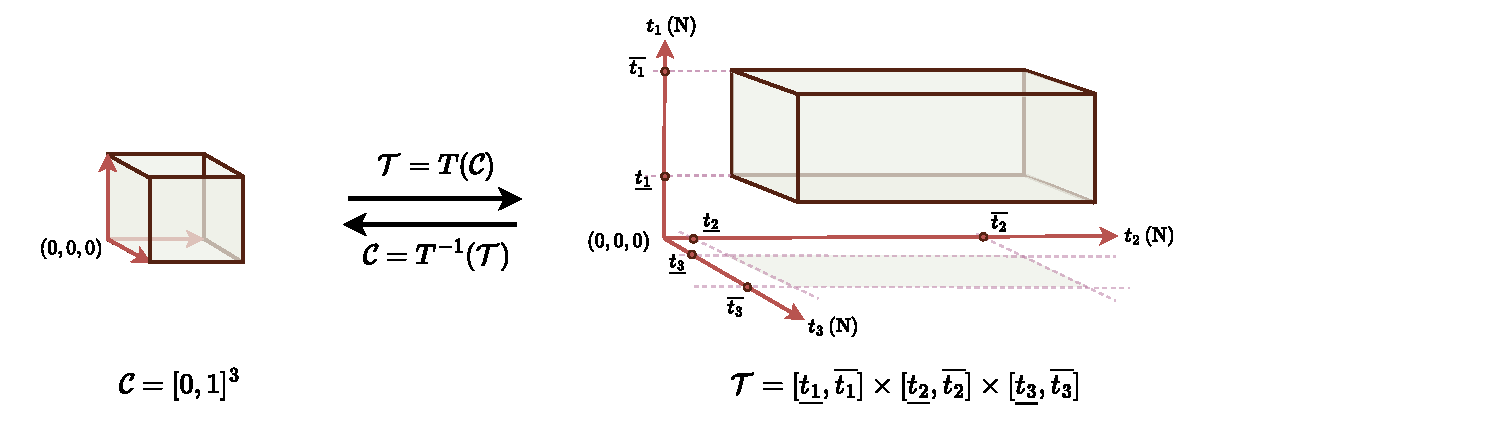
\includegraphics[trim={20 20 150 0}, clip, width=1\linewidth]{img/chapter_2/invertible_transformation.pdf}
    \caption[]{To consider the torque feasible set as a projection of the unit cube $\mathcal{C}=[0,1]^3$, consider the invertible affine transformation $T\,\colon \IR^3 \to \IR^3$ defined as:
    \begin{minipage}{\linewidth}
      \begin{align*}
        T(\mathbf{t}) &= D\mathbf{t} + \underline{\mathbf{t}}, \quad \text{for } D = \begin{pmatrix}
          \overline{t_1} - \underline{t_1} & 0 & 0 \\
          0 & \overline{t_2} - \underline{t_2} & 0 \\
          0 & 0 & \overline{t_3} - \underline{t_3}
        \end{pmatrix} \text{ and } \underline{\mathbf{t}} = \begin{pmatrix}
          \underline{t_1} \\ \underline{t_2} \\ \underline{t_3}
        \end{pmatrix}
      \end{align*}
    \end{minipage}

    Thus, $\mathcal{T} = T(\mathcal{C})$ and the torque feasible set is described as 
    $\left\{\tau \in \IR^3 \mid -LD\mathbf{t} -L\underline{\mathbf{t}} - \mathbf{G},\quad \mathbf{t}\in\mathcal{C}\right\}$, which is clearly an affine projection of a cube, so it is a zonotope by definition.}
    \label{fig:invertible_transfo_cube_orthotope}
  \end{minipage}
\end{figure}

Zonotopes have multiple possible representations, including a non-squared matrix, a set of vertices, delimiting hyperplanes, or even \emph{cells}, which characterize the cube vertices whose projections are the zonotope vertices. Several algorithms exist to transition from one representation to another, the goal of which is to be efficient in time and space. This chapter offers a new perspective on representing zonotopes using their edges and describes an algorithm to compute them directly from a matrix representation of a zonotope. To achieve this goal, let's first delve into zonotope formalism.

For two sets of vectors $A$ and $B$ in $\IR^n$, their \emph{Minkowski sum}, denoted $A\bigoplus B$, is defined as $A\bigoplus B = \left\{ a+b\in \IR^n \mid a\in A,\, b\in B\right\}$. 
Let $\Zono \subset \IRn$ be an $n$-zonotope, \emph{i.e.}, 
the Minkowski sum of $n$-dimensional segment vectors $\Zono = \mathbf{c} + \bigoplus_{i=1}^m \alpha_i \mathbf{g}_i$, where $\mathbf{c} \in \IRn$, $\mathbf{g}_i \in \IRn$ for $i=1,\dots,m$ such that all the $\mathbf{g}_i$ span $\IRn$, and $\alpha_i\in[0,1]$. This corresponds to the following set:
\begin{align*}
  \Zono &= \left\{ \mathbf{z} \in \IR^n \mid \mathbf{z} = \mathbf{c} + \sum_{i=1}^m \alpha_i \mathbf{g}_i,\quad \alpha_i \in [0,1],\, \mathbf{c}, \mathbf{g}_1,\cdots,\mathbf{g}_m\in\IR^n \right\}
\end{align*}

The vectors $\mathbf{g}_i$ are called \emph{generators} and are usually concatenated into the columns of a matrix $G\in\IRnm$. For conciseness, a zonotope is denoted directly using its translation and its generators as $\Zono(\mathbf{c}, G)$, or $\Zono(G)$ if there is no translation. The notation $\Zono(n, m)$ is also convenient to directly refer to the size of the matrix $G$. The generators are assumed to be non-null, and any combination of $n$ of them is assumed to span $\IRn$. In this case, the generators are said to be in \emph{general position}.

\begin{figure}[!htb]
  \captionsetup{justification=centering}
  \begin{minipage}{0.49\linewidth}
    \centering
    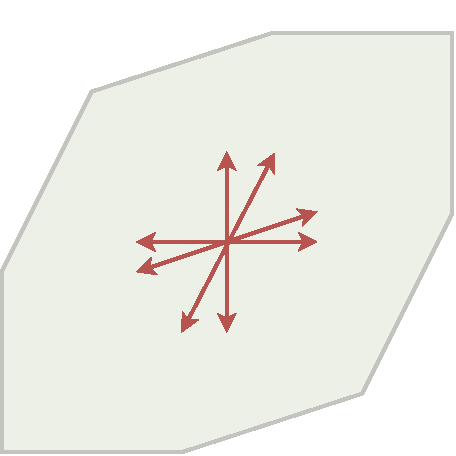
\includegraphics[trim={0 0 0 0},clip, width=0.6\linewidth]{img/chapter_2/zonotope_2d_4g.pdf}
  \end{minipage}
  \hfill
  \begin{minipage}{0.49\linewidth}
    \centering
    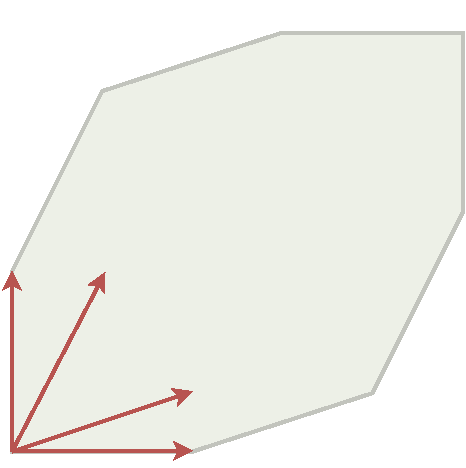
\includegraphics[trim={0 0 0 0},clip,width=0.6\linewidth]{img/chapter_2/zonotope_2d_4g_alt.pdf}
  \end{minipage}
  \caption{Both constructions lead to the same 2D zonotope generated by $4$ generators: the differences lie in the bounds defined for $\alpha_i$, which are $[-1,1]$ for the left zonotope and $[0, 1]$ for the right, and the center $\mathbf{c}$.}
  \label{fig:a_simple_zonotope}
\end{figure}

A zonotope is a specific type of convex polytope; therefore, it can be described via its vertices ($\mathcal{V}$-representation) or a set of inequalities ($\mathcal{H}$-representation), as shown in Figure \ref{fig:zonotope_vertices_hyperplanes}. Several zonotope applications include their use as bounding volumes in collision detection (\cite{guibasZonotopesBoundingVolumes}), as bounds for disturbances and measurement errors (\cite{scottInputDesignGuaranteed2014}), and in approximating the domain of a function of several variables (\cite{stinsonRandomizedAlgorithmEnumerating2016}). More recently in robotics, a neural network was used to predict a path of reachable sets in an environment crowded with dynamic obstacles modeled as zonotopes (\cite{shamsahSociallyAcceptableBipedal2024}).

\begin{figure}[!htb]
  \captionsetup{justification=centering}
  \begin{minipage}{0.49\linewidth}
    \centering
    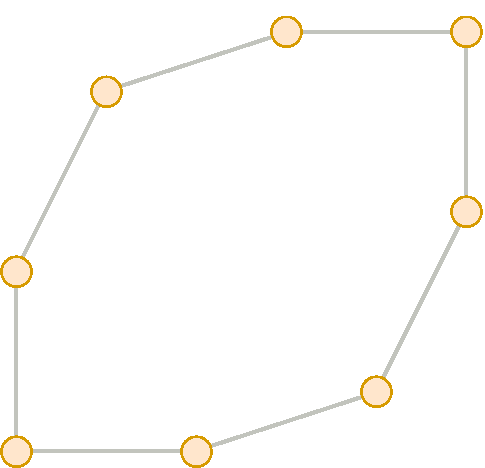
\includegraphics[trim={0 0 0 0},clip, width=0.6\linewidth]{img/chapter_2/zonotope_vertices.pdf}
  \end{minipage}
  \hfill
  \begin{minipage}{0.49\linewidth}
    \centering
    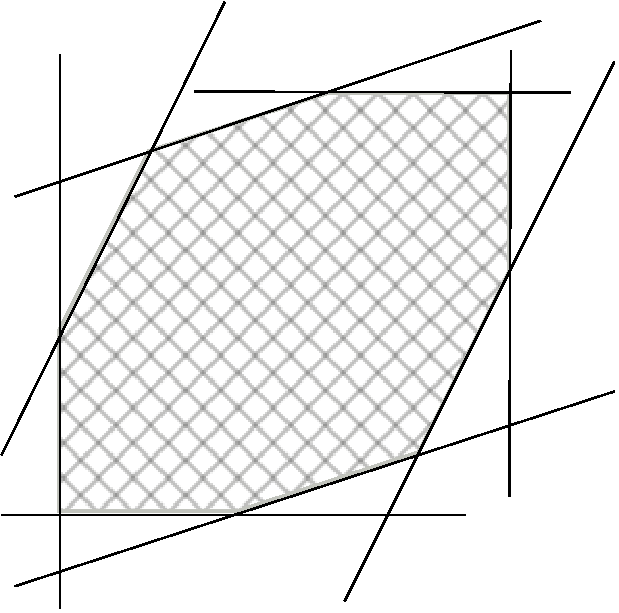
\includegraphics[trim={0 0 0 0},clip,width=0.75\linewidth]{img/chapter_2/zonotope_hyperplanes.pdf}
  \end{minipage}
  \caption{A zonotope can be represented by its vertices or its bounding hyperplanes. The vertex representation defines the zonotope as the convex hull of its vertices (including all interior and surface points). The hyperplane representation defines the zonotope as the intersection of half-spaces so that the direction of the half-space must be specified.}
  \label{fig:zonotope_vertices_hyperplanes}
\end{figure}

The process of retrieving zonotope vertices from its generator representation is a combinatorial problem known as the \emph{vertex enumeration problem}. The explicit enumeration of zonotope vertices is required in applications such as the fixed-rank integer quadratic program (\cite{ferrezSolvingFixedRank2005a}), signal processing (\cite{markopoulosOptimalAlgorithmsL_12014}), and linear regression models with interval data (\cite{cernyPossibilisticApproachLinear2013}).

Unfortunately, converting zonotope generators to vertices or bounding hyperplanes is a combinatorial problem. As the dimension or the number of generators increases, the number of vertices increases rapidly: Theorem 3.1 from (\cite{ferrezSolvingFixedRank2005a}) states that the number of vertices of an $n$-zonotope $\mathcal{Z}$ with $m$ generators is $\leq 2 \sum_{i=0}^{n-1} \binom{m-1}{i}$, with equality satisfied when the generators are in general position. For instance, a 3D zonotope can have up to $92$ vertices if it is defined by $10$ generators; $2452$ if it has $50$ generators; and $9902$ vertices for $100$ generators. Similarly, for an $n$-zonotope with $50$ generators, it has up to $39300$ vertices for $n=4$, more than $5.6\times 10^{14}$ for $n=25$, and more than $1.1\times 10^{15}$ for $n=50$. In a biomechanical context, considering the Stanford upper limb musculoskeletal model consisting of $50$ muscles and $7$ degrees-of-freedom (\cite{holzbaurModelUpperExtremity2005}), the torque feasible set has at most $32244452\approx 3.2\times 10^{7}$ vertices. Consequently, the required space to describe all the vertices becomes large very quickly, regardless of the efficiency of the enumeration algorithm. 

The following Section \ref{edge_enumeration_algorithm_section} presents a novel, efficient zonotope edge enumeration algorithm, called \emph{EdgeEnum}, which can be used to enumerate the vertices of a zonotope. Section \ref{time_complexity_edgeenum} shows that EdgeEnum is indeed theoretically \emph{efficient} by proving the polynomiality of both its time and space complexity when $n$ is fixed. An asymptotic growth comparison is also performed with various recent enumeration algorithms adapted to the zonotope vertex enumeration problem. Section \ref{time_benchmark} compares the time benchmarks of multiple algorithms and demonstrates that, in practice, \emph{exact} enumeration techniques may not be suitable when rapid evaluations of zonotopes are required, as we need for Chapters \ref{chapter:3} and \ref{chapter:4} for an optimization-based muscle personalization process. In this regard, Section \ref{sec:approximation_of_vertices_zonotope} offers some insights into the computation time of approximated vertex enumeration algorithms. Finally, Section \ref{conclusion_zonotope_enum_algorithm} summarizes the results and advantages offered by our approach, such as the ease of implementation and the potential for parallelism compared to existing methods, while highlighting the effectiveness of using vertices to describe zonotope characteristics of interest such as its global shape and orientation.

\section{The edge enumeration algorithm}
\label{edge_enumeration_algorithm_section}

While the main goal is to enumerate zonotope vertices, this section presents first an algorithm that enumerates the edges of a zonotope and then describes an edge-to-vertex conversion algorithm with negligible additional computation time. The edge enumeration algorithm takes as input the generator matrix of an $n$-zonotope $\Zono$ with $m$ generators in general position and returns a set of $m$-cube edges that map to the edges of $\Zono$.

Vertices do not contain information about other vertices, whereas edges are linked to at least two vertices. Therefore, knowledge of an edge allows for the description of its extremal vertices. This novel approach uses this information to make vertex enumeration faster by enumerating zonotope edges. Since a zonotope is the projection of a higher-dimensional cube, its edges are also the projection of some cube edges.

\subsubsection*{From cube edges to zonotope edges}
The construction of the edges of an $m$-dimensional hypercube, also called an $m$-cube, is an iterative process over dimensions 2 to $m$ (Figure \ref{fig:cube_edge_construction}). Starting from a square (or the 2-cube), each of its edges is embedded in 3D and then duplicated and translated by 1 along the newly created dimension.  New edges arise from this duplication: for each vertex $v$ in the previous step, a segment is created between $v$ and its newly duplicated and translated version $v'$. This process is iterated until the $m^{\text{th}}$ dimension is reached, at which point all of the $m$-cube edges are enumerated.

\begin{figure}[!htb]
  \captionsetup{justification=centering}
  \centering
  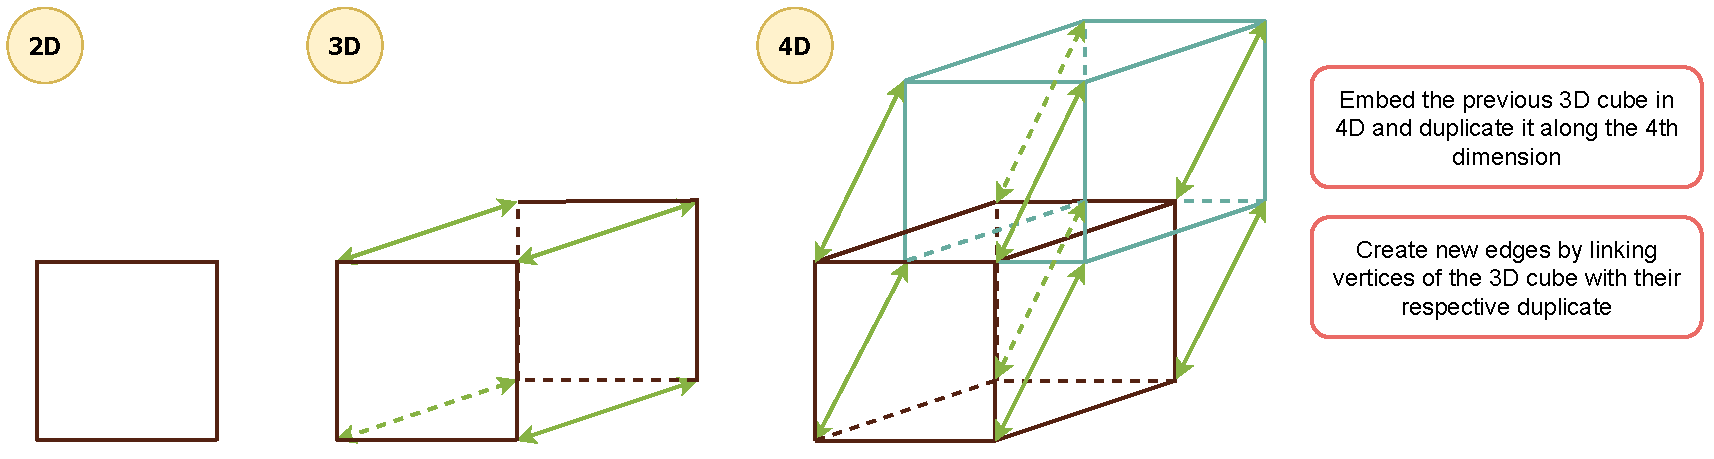
\includegraphics[trim={0 0 0 0},clip, width=1.0\linewidth]{img/chapter_2/zonotope_construction_from_cube_edge_duplication.pdf}
  \caption{Constructing the edges of a zonotope with $4$ generators requires constructing the edges of a $4$-dimensional hypercube. The process is iterative and starts from the square to retrieve the cube, then the $4$-cube. The creation of new edges arising at each new step is indicated by the green double arrows.}
  \label{fig:cube_edge_construction}
\end{figure}

Once all $m$-cube edges are enumerated, projecting them through the generator matrix of the zonotope yields a result similar to Figure \ref{fig:from_cube_edges_to_zonotope_edges}: a collection of line segments appear to encapsulate the zonotope.

\begin{figure}[!htb]
  \captionsetup{justification=centering}
  \centering
  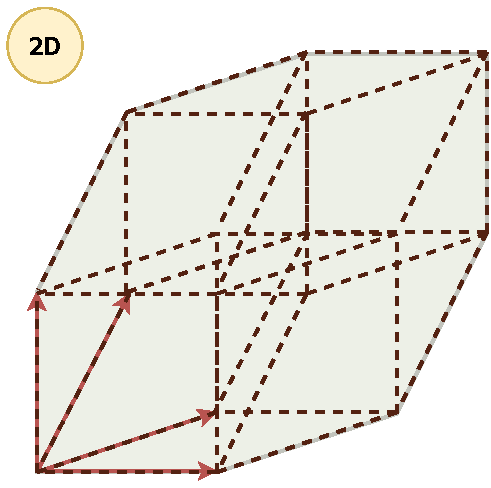
\includegraphics[trim={0 0 0 0},clip, width=0.3\linewidth]{img/chapter_2/zonotope_after_cube_duplication.pdf}
  \caption{Projecting the $4$-cube edges through the generator matrix of a 2D zonotope with $4$ generators.}
  \label{fig:from_cube_edges_to_zonotope_edges}
\end{figure}

This phenomenon is due to a parallelism property specific to zonotopes. Two segments or lines are \emph{parallel} if their direction vectors are collinear.

\begin{lemmabox}{Parallelism of zonotope edges with the generators}{zono_edges_parallel}
  For any $n$-dimensional zonotope $\Zono \subset \IRn$ with $m$ generators, each of its edges is parallel to one of its generators.

  Moreover, each projected edge of the $m$-cube is also parallel to one of the generators.
\end{lemmabox}
\begin{proof}
A linear or affine map preserves parallelism. 
Consider a zonotope $\Zono$ described by generators $\mathbf{g}_1,\dots,\mathbf{g}_m \in \IRn$ in general position. Let $G$ denote the generator matrix. If $n\geq 2$, then the edges of the $m$-cube clearly surject onto the zonotope edges.
The edges of the $m$-cube can be grouped by parallelism with a representing vector $\mathbf{r}_i = e_i \in \IRm$, where $e_i$ corresponds to the $i^{\text{th}}$ vector of the canonical basis of $\IRm$. Thus, $G\mathbf{r}_i = \mathbf{g}_i$. This ensures that when a cube edge is projected through $G$, it will necessarily be parallel to one of the generators.
\end{proof}

\begin{figure}[!htb]
      \captionsetup{justification=centering}
      \begin{minipage}{0.49\linewidth}
        \centering
        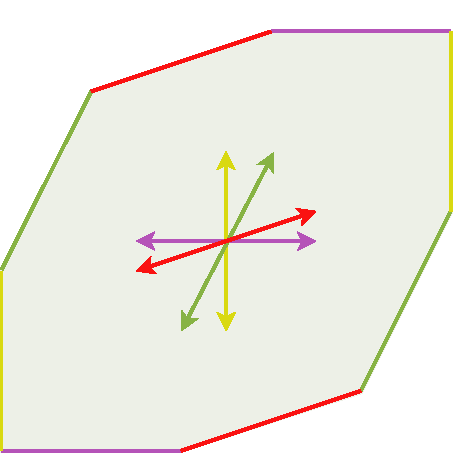
\includegraphics[trim={0 0 0 0},clip, width=0.55\linewidth]{img/chapter_2/zonotope_edges_parallel_generator.pdf}
      \end{minipage}
      \hfill
      \begin{minipage}{0.49\linewidth}
        \centering
        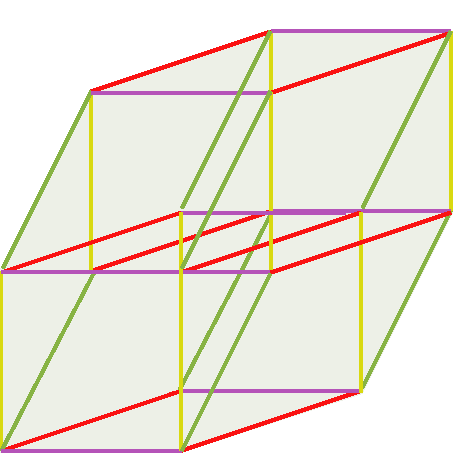
\includegraphics[trim={0 0 0 0},clip,width=0.55\linewidth]{img/chapter_2/zonotope_edges_parallel_generator_alt.pdf}
      \end{minipage}
      \caption{Left: Each edge of a zonotope $\Zono$ is parallel to one of its generators. Right: Projecting a $4$-cube edge through the generator matrix of $\Zono$ produces a line segment parallel to one of the generators.}
      \label{fig:zonotope_edges_parallel}
    \end{figure}
    
To enumerate the edges of a zonotope $\Zono(\mathbf{c}, G)$, a naive approach would be to first consider each edge $\mathbf{e}$ of an $m$-cube and project it through $\mathbf{e} \mapsto \mathbf{c} + G\mathbf{e}$. Then, after a selection process, only a relevant subset of these projected edges would be considered. However, this involves computing \emph{all} edges of an $m$-cube, which is not feasible due to the high combinatorics involved in the number of possible edges. Indeed, this would amount to $m2^{m-1}$ edges, which is greater than $2^m$, the number of its vertices (\cite{grunbaumConvexPolytopes2013}).

Our novel approach consists of using a straightforward elimination technique directly from the cube space, to remove unnecessary cube edges that do not project onto zonotope edges. The following paragraphs describe this process.

\subsubsection*{The convex hull of parallel lines}
As established in Lemma \ref{th:zono_edges_parallel}, each edge of a zonotope is parallel to one of its generators. Furthermore, each edge of the $m$-cube maps to a segment parallel to a generator. This allows for grouping the projected cube edges by parallelism, with a generator serving as the group representative. For each group, the extremal segments define the edges of the zonotope parallel to the considered generator.

Given these grouped projected edges, the next question is: \emph{how can we select only those on the zonotope surface?} While this is a challenging question for an arbitrary set of segments, the fact that we are working with projected edges parallel to a generator simplifies the problem.

This selection process is termed the \emph{convex hull of parallel lines}.  While convex hull algorithms are typically implemented for sets of points, the parallelism in this case allows for a modified approach that leverages the classic convex hull of points.

To illustrate this, consider a 2D example that generalizes to any dimension.  In the first iteration of the algorithm, the edges of a square are created, embedded in 3D, and projected through the submatrix of $G$ consisting of the first two columns. This results in three groups of edges, as shown by the edge colors in Figure \ref{fig:convex_hull_lines_intro}.

\begin{figure}[!htb]
  \captionsetup{justification=centering}
  
  \centering
  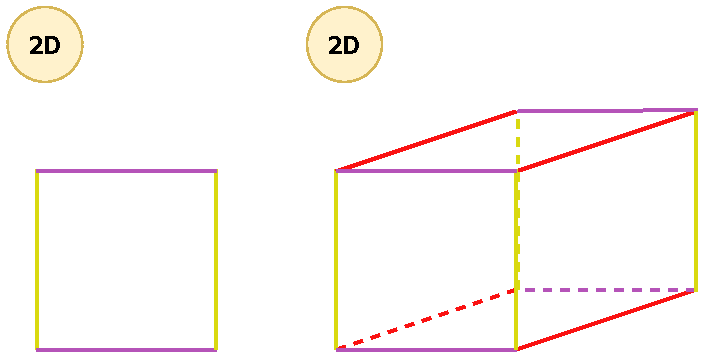
\includegraphics[trim={0 0 0 0},clip,width=0.5\linewidth]{img/chapter_2/zonotope_convex_hull_lines_intro.pdf}

  \caption{The edges on the right are created from embedding and duplicating the square edges to create a cube and then projecting them onto the plane through the first two columns of $G$.}
  \label{fig:convex_hull_lines_intro}
\end{figure}

Consider a group of parallel edges, such as the purple ones in Figure \ref{fig:convex_hull_lines_intro}, and extend them to lines. An arbitrary point is selected in the zonotope space and projected orthogonally onto each line. These projected points span a space of at most $n-1$ dimensions, where $n$ is the dimension of the zonotope. The convex hull operation is then applied to this set of projected points, and only the edges associated with points on the convex hull are retained (cf. Figure \ref{fig:convex_hull_lines}).

% \clearpage
\begin{figure}[!htb]
  \captionsetup{justification=centering}
  
  \centering
  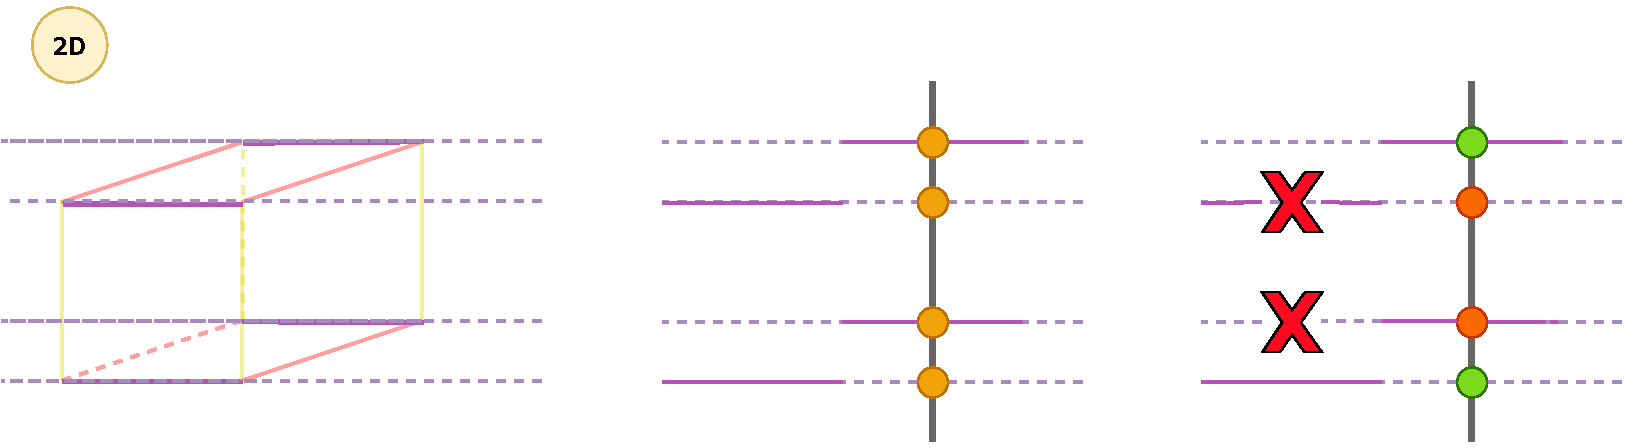
\includegraphics[trim={0 0 0 0},clip,width=1\linewidth]{img/chapter_2/zonotope_convex_hull_lines.pdf}

  \caption{From left to right: A group of parallel edges is selected and extended to lines. An arbitrary point is projected orthogonally onto these lines. The convex hull operation is applied to these points to retrieve the associated extremal edges. This works in any dimension, as long as a set of parallel lines is considered.}
  \label{fig:convex_hull_lines}
\end{figure}

This process is repeated for all groups of edges, which corresponds to the number of dimensions of the underlying hypercube, as shown in Figure \ref{fig:convex_hull_lines_repeat_groups}.

\begin{figure}[!htb]
  \captionsetup{justification=centering}
  
  \centering
  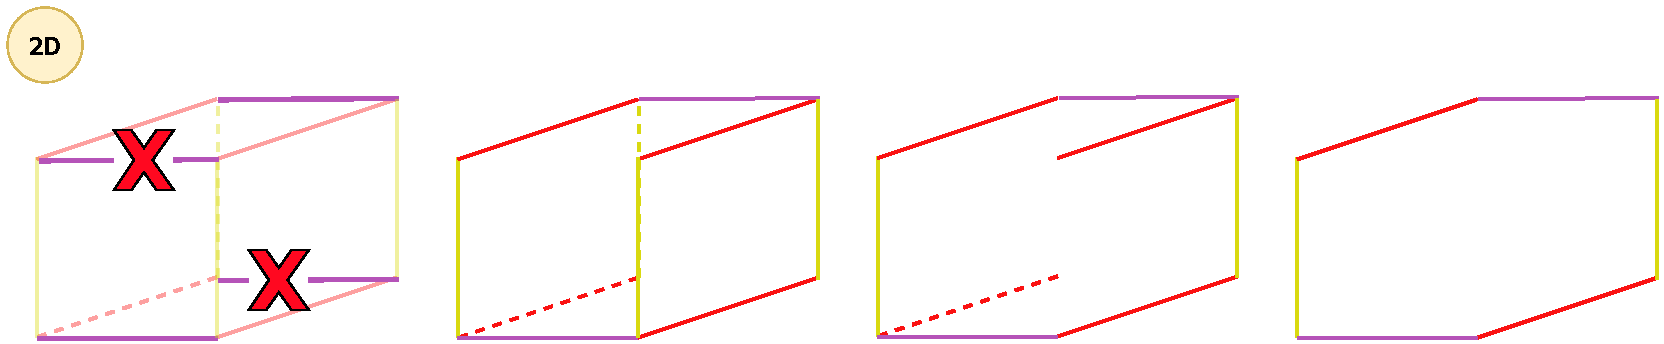
\includegraphics[trim={0 0 0 0},clip,width=1\linewidth]{img/chapter_2/zonotope_edge_elimination_repeat.pdf}

  \caption{Selection of the extremal edges for each group of parallel edges by applying the convex hull of parallel lines. First purple edges, then yellow, and finally red.}
  \label{fig:convex_hull_lines_repeat_groups}
\end{figure}

Once all groups have been processed, the remaining edges are precisely those needed to produce the edges of the zonotope generated by the first three columns of $G$. The embedding, duplication, and translation process is then employed to create the new edges in 4D, which are projected through the submatrix of $G$ consisting of the first four columns. The algorithm terminates when, after multiple iterations, the selected cube edges belong to the $m$-cube (cf. Figure \ref{fig:zonotope_edges_elimination_end}).

\begin{figure}[!htb]
  \captionsetup{justification=centering}
  
  \centering
  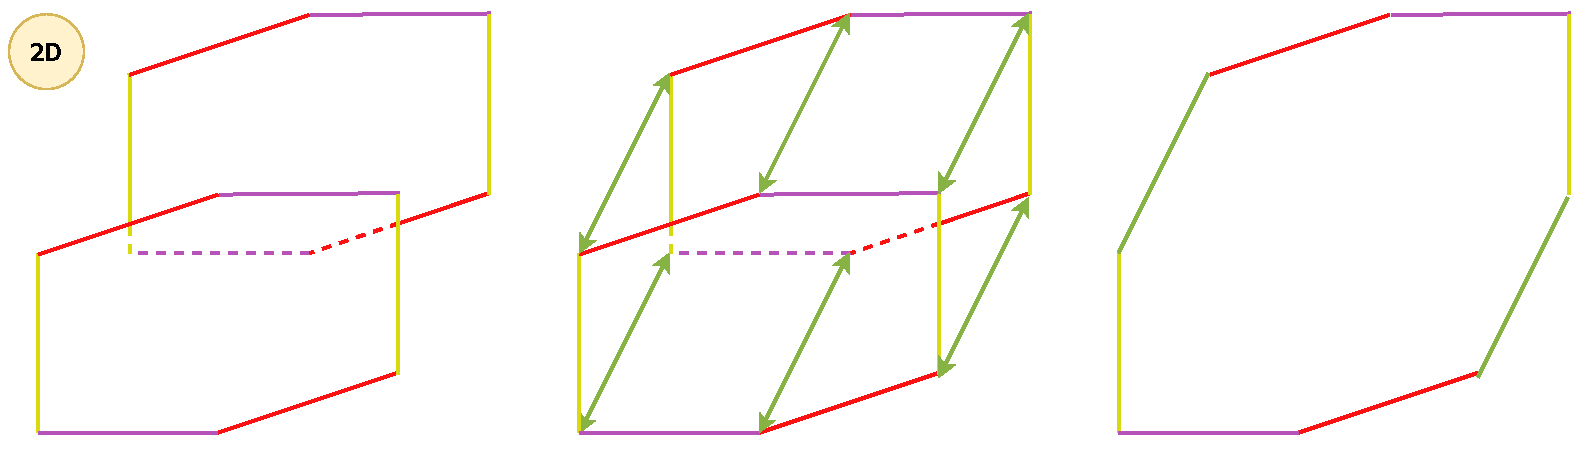
\includegraphics[trim={0 0 0 0},clip,width=1\linewidth]{img/chapter_2/zonotope_edges_elimination_end.pdf}

  \caption{After exactly $m-2$ iterations, the returned edges are precisely the zonotope edges.}
  \label{fig:zonotope_edges_elimination_end}
\end{figure}


\clearpage 
\subsubsection*{The EdgeEnum algorithm}

In the following algorithms, an edge of the $m$-cube is represented by two $m$-dimensional vectors: a direction vector and an initial position vector. Algorithm \ref{alg:cube_edge_enumeration} details the creation of a new set of edges in a higher dimension ($d+1$) from a given set of edges in $\mathbb{R}^d$, based on the construction of edges of a higher-dimensional cube. Algorithm \ref{alg:edge_enum}, called EdgeEnum, constructs zonotope edges following the reasoning described previously.

\begin{figure}[!ht]
  \centering
  \begin{minipage}{1.0\linewidth}
    \begin{algorithm}[H]
      \SetAlgoLined
      \KwData{$\textup{E}_d$, a set of edges in $\mathbb{R}^d$}
      \KwResult{$\textup{E}_{d+1}$, a set of edges in $\mathbb{R}^{d+1}$}
      
      \SetKwFunction{FMain}{duplicateAndLinkEdges}
      \SetKwProg{Fn}{Function}{:}{}
      \Fn{\FMain{$\textup{E}_d$}}{
        $\text{E}_{d+1} \gets \emptyset$\;
        \ForEach{$\mathbf{e}\in \textup{E}_d$}{
          $\mathbf{e}_0 \gets \textup{embedInOneHigherDimension}(\mathbf{e})$\;
          $\mathbf{e}_1 \gets \textup{translateAlongNewDimensionBy1}(\mathbf{e}_0)$\;
          $v_0^1,\, v_0^2 \gets \textup{verticesAtExtremities}(\mathbf{e}_0)$\;
          $v_1^1,\, v_1^2 \gets \textup{verticesAtExtremities}(\mathbf{e}_1)$\;
          $\mathbf{e}_{01}^1 \gets \textup{createEdge}(v_0^1, v_1^1)$\;
          $\mathbf{e}_{01}^2 \gets \textup{createEdge}(v_0^2, v_1^2)$\;
          $\text{E}_{d+1} \gets \text{E}_{d+1} \cup \{\mathbf{e}_0, \mathbf{e}_1, \mathbf{e}_{01}^1, \mathbf{e}_{01}^2\}$;
        }    
        \Return{$\textup{E}_{d+1}$}
      }
      \textbf{End Function}
      \caption{Duplication, translation, and linking of edges}
      \label{alg:cube_edge_enumeration}
    \end{algorithm}
  \end{minipage}
\end{figure}

\begin{figure}[!ht]
  \centering
  \begin{minipage}{1.0\linewidth}
    \begin{algorithm}[H]
      \SetAlgoLined
      \KwData{A matrix $N \in \mathbb{R}^{n\times m}$, with $n\geq 2$ and $m\geq 2$}
      \KwResult{Edges of the zonotope $\Zono(\mathbf{c}, N)$}
      $d\gets 2$\;
      $N_d\gets N[:,:d]$\;      
      $\text{Edges}(\Cube_d)\gets \{\text{edges of the 2D cube}\}$ \tcp*{where $\Cube_d$ is the cube $[0,1]^d$.}
      $\text{Edges}(\Zono(\mathbf{c}, N_d))\gets \{\mathbf{c} + N_d\mathbf{e} \mid \mathbf{e}\in\text{Edges}(\Cube_d)\}$ \;
      
      $d\gets 3$\;
      \While{$d \leq m$}{
        $N_d\gets N[:,:d]$\;
        $\text{Edges}(\Cube_{d-1}) \gets \text{Edges}(\Cube_d)$\;
        $\textup{Edges}(\Cube_{d}) \gets \textup{duplicateAndLinkEdges}(\textup{Edges}(\Cube_{d-1}))$ \tcp*{cf. Algorithm \ref{alg:cube_edge_enumeration}}
        
        $\text{Edges}(\Zono(\mathbf{c}, N_d))\gets \{\mathbf{c} + N_d\mathbf{e} \mid \mathbf{e}\in\text{Edges}(\Cube_d)\}$ \;
    
        \ForEach{group of parallel edges $G\in\textup{Edges}(\Zono(\mathbf{c}, N_d))$}{
          \ForEach{$\mathbf{c} + N_d\mathbf{e} \notin \textup{ext}(\textup{conv}(G))$}{
            $\text{Edges}(\Cube_d) \gets \text{Edges}(\Cube_d) / \{\mathbf{e}\}$\;
          }
          
        }
        
        $d\gets d+1$
      }
      
      $\text{Edges}(\Zono(\mathbf{c}, N_d))\gets \{\mathbf{c} + N_d\mathbf{e} \mid \mathbf{e}\in\text{Edges}(\Cube_d)\}$ \;
      \Return{$\textup{Edges}(\Cube_d),\, \textup{Edges}(\Zono(\mathbf{c}, N_d))$}
      \caption{EdgeEnum: zonotope edge enumeration algorithm}
      \label{alg:edge_enum}
    \end{algorithm}

  \end{minipage}
\end{figure}

\section{Theoretical complexity}
\label{time_complexity_edgeenum}
This section presents various theoretical results about the new algorithm, using computational complexity as the primary tool for comparison. While a thorough analysis of time and space complexity is provided, the primary focus is on the asymptotic time growth as the number of generators increases, as this relates to a larger number of muscles considered when computing the torque feasible set. Therefore, $n$, the dimension of the ambient space of the zonotope, is considered to be fixed, while the number of generators, $m$, is assumed to be large.

Before delving into the analysis, let's review some basic concepts related to algorithmic complexity and asymptotic growth:

\paragraph*{Asymptotic Growth and Big O Notation.} Asymptotic growth describes the behavior of a function as its input becomes very large. The Big O notation denotes the dominant terms of a function. For instance, the function $f\colon \mathbb{N} \rightarrow \mathbb{N}$ defined by $f(n) = 4n^5 + n^5\log (n)$ is dominated by the term $n^5\log(n)$. This means that as $n$ tends to $+\infty$, $f(n)$ will have approximately the same growth rate as the function $n\mapsto n^5\log(n)$. The Big O notation expresses this comparison by stating that $f$ is in $O(n^5\log(n))$ or $f(n) = O(n^5\log(n))$. To compare the asymptotic growth of two functions, their respective growth rates are calculated, and the ratio of these rates is evaluated to determine which function has slower growth. If the ratio tends to a constant value, then both functions have asymptotically the same growth. More generally, $O$ represents a class of functions bounded by a given formula. In the example above, $f$ is \emph{in} $O(n^5\log(n))$, but it is also in higher classes such as $O(n^6)$ or $O(n^{20})$.

\paragraph*{Algorithmic Complexity.} Two types of complexity are commonly used to describe algorithms: \emph{time} complexity and \emph{space} complexity. Time complexity theoretically evaluates the time required for each operation, while space complexity evaluates the required storage.

\paragraph*{Efficient Algorithm.} An algorithm is \emph{polynomial} or \emph{efficient} if its time complexity is upper bounded by a polynomial expression of both the input size and the output size (\cite{fukudaZonotopeConstructionMinkowski2004a}). In other words, the running time of the algorithm does not grow exponentially as the input size increases, making it generally efficient for solving problems. For algorithms related to zonotope vertex enumeration, the input size corresponds to the number of dimensions times the number of generators (essentially the number of elements in the generator matrix), while the output size includes the number of vertices, faces, and generator dimensions.

\paragraph*{Compact Algorithm.} An algorithm is \emph{compact} if its space complexity is polynomial in the input size. This means that a compact algorithm does not store \emph{all} of the output and can stream the results directly without storing the entire output. This is a valuable property, especially when the output size is large. In the literature, two main approaches can be found: reverse-search-based algorithms and iterative algorithms. Algorithms are theoretically more valuable if they are compact, especially in high dimensions, so this approach is preferred and commonly found (\cite{avisPivotingAlgorithmConvex}; \cite{guCounterfactualIdentificationLatent2022}; \cite{radaNewAlgorithmEnumeration2018}). However, non-compact algorithms should not be excluded, depending on the application context.

\paragraph*{Optimal Algorithm.} An algorithm is \emph{optimal} (in time and/or in space) if its complexity has been proven to be the lowest possible. For instance, Theorem 3.2 in (\cite{ferrezSolvingFixedRank2005a}) states that a time-optimal algorithm exists that enumerates all zonotope vertices in time $O(m^{n-1})$, which was implemented in (\cite{edelsbrunnerConstructingArrangementsLines1983}). However, such an optimal algorithm may not be practical (\cite{ferrezSolvingFixedRank2005a}). First, it uses an incremental strategy that requires storing all extreme points of a subproblem based on a smaller number of generators. Second, it is complex to implement and needs to store all faces and their incidence (i.e., whether the intersection of two faces is another face). In other words, Edelsbrunner et al.'s algorithm is time-optimal and efficient but space-inefficient.

This work focuses primarily on time efficiency. As the following theorems demonstrate, the new algorithm is time-efficient, even when considering the edge-to-vertex transition. It is also space-efficient but not compact.

Before analyzing the complexity, let us introduce a useful result concerning the number of specific faces in a zonotope. A zonotope $\Zono$ in dimension $n$ has $n-1$ types of faces: the $0$-faces are called \emph{vertices}, the $1$-faces \emph{edges}, the $(n-2)$-faces \emph{ridges}, and the $(n-1)$-faces \emph{facets}. In specific cases, such as in dimension 2, the edges correspond to the facets. In 3D, edges correspond to ridges.

\begin{lemmabox}{Upper bound on the number of $k$-faces of a zonotope}{nb_k_faces_zonotope}
  For $G\in\IRnm$, the number of $k$-faces of the zonotope $\Zono(G)$ for $k=1,\dots, n-1$ is upper bounded by $f_k(\Zono)$, where
  \[f_k(\Zono) = 2\binom{m}{k} \sum_{i = 0}^{n-k-1} \binom{m-k-1}{i}.\]
  This bound is attained if $\Zono$ is in general position.
\end{lemmabox}
\begin{proof}
  This result, with proof, can be found in (\cite{fukudaZonotopeConstructionMinkowski2004a}; \cite{donohoCountingFacesRandomlyProjected2010}; \cite{grunbaumConvexPolytopes2013}).
\end{proof}

\subsection{Time complexity}
\begin{theorembox}{Time complexity of EdgeEnum}{time_complexity}
  For an $n$-zonotope $\Zono$ with $m$ generators in general position, the edge enumeration algorithm has time complexity
  \[O\left( nm^2f_1(\Zono)\right),\]
  where $f_1(\Zono)$ denotes the number of edges of $\Zono$.
\end{theorembox}
\begin{proof}
    Each iteration of the algorithm (i.e., $d=3,\dots, m$) considers a new zonotope $\Zono_d$ generated by the first $d$ columns of the generator matrix $G\in\IRnm$ and constructs its edges based on the set of edges of $\Zono_{d-1}$. The following is a thorough analysis of the computation time of each step in the algorithm:

    \textbf{1. Embed, duplicate, and translate Edges:} In the first inner loop, a new dimension is added to the edges of $\Zono_{d-1}$. This is achieved by concatenating a $0$ to both the direction and position vectors that describe each edge. These embedded edges are then duplicated, and the copied versions have their direction and position last coordinates mutated to $1$. New edges are created by linking the corresponding extremity points from the embedded edges to their translated counterparts. This entire step can be performed in $O(1)$ time complexity for each substep, within a loop over each of the previous edges, resulting in $O(f_1({\Zono_{d-1}}))$ time complexity.

    \textbf{2. Group edges by parallelism:} The newly created set of edges consists of exactly $4f_1(\Zono_{d-1})$ edges. Since collinearity between cube edges is preserved under linear transformation, grouping edges of zonotope $\Zono_d$ by parallelism only requires grouping the cube edges by their directions. Using a dictionary structure in Python, this grouping process has a time complexity of $O(f_1(\Zono_{d-1}))$.
    
    \textbf{3. Apply the convex hull to each group of edges:} Each group of edges consists of $2f_1(\Zono_{d-1}) / (d-1)$ edges, and there are $d$ groups. For each group, each edge is projected onto $\IRn$ through the generator matrix of $\Zono_d$. This corresponds to one matrix-vector operation with a time complexity of $O(nd)$ per edge. After the projection, the orthogonal projection of the origin in $\IRn$ onto the line spanned by the projected edge is computed in $O(n)$ time complexity (the dimension of the ambient space where the line is defined). The convex hull of the projected edges is then computed as the convex hull of the orthogonal projections of the origin onto the lines spanned by the edges. Consider the time complexity of Chan's convex hull algorithm in $n$ dimensions. It is an output-sensitive algorithm, meaning its complexity depends on the size of the output. Its time complexity is $O(n_v\log h)$, with $n_v$ being the number of given points and $h$ the number of points on the convex hull. Since the zonotope $\Zono_d$ is in general position, the number of edges in each group is $f_1(\Zono_d) / d$. The total time complexity of step 3 is then of order 
    $d (\frac{2f_1(\Zono_{d-1})}{d-1}nd + \frac{2f_1(\Zono_{d-1})}{d-1}n + \frac{2f_1(\Zono_{d-1})}{d-1}\log(\frac{f_1(\Zono_{d})}{d}))$, which is
    $O(f_1(\Zono_{d-1}) nd +f_1(\Zono_{d-1})  \log(f_1(\Zono_{d}) / d))$.

    After $d$ iterations, the complexity is of order $\sum_{d=3}^m f_1(\Zono_{d-1}) nd +  f_1(\Zono_{d-1}) \log(f_1(\Zono_d) / d)$ and since $d \leq m$ and $f_1(\Zono_d) \leq f_1(\Zono)$, we have the following upper bound:
    \begin{align*}
        \sum_{d=3}^m f_1(\Zono_{d-1}) nd +  f_1(\Zono_{d-1}) \log(f_1(\Zono_d) / d) &\leq  f_1(\Zono) \left[ n \sum_{d=3}^m d + \sum_{d=3}^m \log\left(\frac{f_1(\Zono)}{d}\right) \right] \\
        &\leq  f_1(\Zono) \left[ nm\frac{m+1}{2} +  \log\left(\prod_{d=1}^m\frac{f_1(\Zono)}{d}\right) \right] \\
        &\leq  f_1(\Zono) \left[ n\frac{m^2+m}{2} +  \log\left(\frac{f_1(\Zono)^m}{m!}\right) \right]
    \end{align*}
    So the edge-based algorithm is upper bounded in $O\left( nm^2f_1(\Zono) +  f_1(\Zono)\log\left(\frac{f_1(\Zono)^m}{m!}\right)\right)$.

    The next step is to show that $nm^2f_1(\Zono)$ is the dominant term in this upper bound. This is done by demonstrating that for any growth of $n$ and $m$, the expression 
    $$f_1(\Zono)\log\left(\frac{f_1(\Zono)^m}{m!}\right) / (nm^2f_1(\Zono))$$
    is upper-bounded by a function whose growth tends to be constant (meaning it is $O(1)$).
    \begin{align*}
        \frac{f_1(\Zono)\log\left(\frac{f_1(\Zono)^m}{m!}\right)}{nm^2f_1(\Zono)} 
        &\leq \frac{1}{nm^2}\log\left(f_1(\Zono)^m\right) \\
        &= \frac{1}{nm}\log\left(f_1(\Zono)\right) \\
        &= \frac{1}{nm} \log\left(2\binom{m}{1}\sum_{i=0}^{n-2}\binom{m-2}{i}\right),\quad \text{using theorem \ref{th:nb_k_faces_zonotope}} \\
        &\leq \frac{1}{nm} \log\left(m2^{m-1}\right),\quad \text{using } \sum_{i=0}^{n-2}\binom{m-2}{i} \leq \sum_{i=0}^{m-2}\binom{m-2}{i} = 2^{m-2}  \\
        &= \frac{ \log(m)}{nm} + \frac{ (m-1)\log(2)}{nm} \\
    \end{align*}
    There are now three cases to study:
    \begin{enumerate}[noitemsep]
        \item {$n \rightarrow +\infty$ and $m$ grows at a smaller rate than $n$ ($\lim_{m,n\to +\infty}\frac{m}{n} = 0$): 
        $$\lim_{m,n\to +\infty}\frac{ \log(m)}{nm} = \lim_{m,n\to +\infty}\frac{1}{nm}  = 0\quad \text{and} \quad \lim_{m,n\to +\infty} \frac{ (m-1)\log(2)}{nm} = \lim_{n\to +\infty}\frac{1}{n}  =  0$$
        }
        \item  {$m \rightarrow +\infty$ and $n$ grows at a smaller rate than $m$ ($\lim_{m,n\to +\infty}\frac{n}{m} = 0$): 
        $$\lim_{m,n\to +\infty}\frac{ \log(m)}{nm} = \lim_{m,n\to +\infty}\frac{1}{nm}  = 0\quad \text{and} \quad \lim_{m,n\to +\infty} \frac{ (m-1)\log(2)}{nm} = \lim_{m,n\to +\infty}\frac{1}{n}  =  0$$
         }
         \item  {$m \rightarrow +\infty$ and $n \rightarrow +\infty$ at an equivalent rate ($\lim_{m,n\to +\infty}\frac{n}{m} = C$, for $C$ a positive constant): 
         $$\lim_{m,n\to +\infty}\frac{ \log(m)}{nm} = \lim_{m,n\to +\infty}\frac{1}{nm}  = 0\quad \text{and} \quad \lim_{m,n\to +\infty} \frac{ (m-1)\log(2)}{nm} = \lim_{m,n\to +\infty}\frac{1}{n}  =  0$$
          }
    \end{enumerate}
    All cases confirm that the growth of $f_1(\Zono)\log\left(\frac{f_1(\Zono)^m}{m!}\right)$ is dominated by the growth of  $nm^2f_1(\Zono)$ for any growth of $m$ and $n$. Therefore, the complexity of the edge enumeration algorithm is $O(nm^2f_1(\Zono))$.
\end{proof}

The following intermediate result will be used in the proof of Theorem \ref{th:time_complexity_n_fixed}.
\begin{lemmabox}{Asymptotic upper bound for the number of $k$-faces}{big_O_nb_k_faces} 
For a zonotope $\Zono$ in dimension $n$ with $m$ generators in general position, the number of $k$-faces of $\Zono$, denoted by $f_k(\Zono)$, has an asymptotic growth upper-bounded by $O(m^{n-1})$ when $k$ and $n$ are fixed, and $m$ is large.
\end{lemmabox}

While it is well-known that the number of vertices $f_0(\Zono)$ is asymptotically bounded by $O(m^{n-1})$ (proven in (\cite{zaslavskyFacingArrangementsFaceCount1975})), this lemma extends this result to higher dimensions to provide an asymptotic upper bound for the number of $k$-faces when $k$ and $n$ are constant. This implies that the number of vertices, edges, ridges, hyperplanes, and all types of $k$-faces of a general zonotope are all upper bounded by the same type of growth as $m$ increases. This lemma will be used later to compute the asymptotic growth of the edge enumeration algorithm when $n$ is fixed, which will facilitate comparison with existing algorithms.
\begin{proof}
    The proof proceeds by finding an upper bound for $f_k(\Zono)$ that is $O(m^{n-1})$ for fixed $n$. First, note that for $0\leq n\leq m$, $m^n$ is an upper bound for $\binom{m}{n}$:
    \begin{align}
    \label{ineq:upper_bound_binomial}
    \binom{m}{n} &= \frac{m!}{n!(m-n)!} = \frac{1}{n!} \cdot m(m-1)(m-2)\dots (m-n+1) \leq m^n.
    \end{align}
      
    Also, when $m$ is large, and $k, n$ are fixed, it is reasonable to assume that $(n-k-1) \leq (m-k-1)/2$, so
    \begin{align}
    \label{ineq:upper_bound_binomial_half}
    \binom{m-k-1}{i}\leq \binom{m-k-1}{n-k-1},\quad \text{for any $i = 1, \dots, n-k-1$}.
    \end{align}
      
    Hence, the following holds:
    \begin{align*}
    f_k(\Zono) &= 2\binom{m}{k}\sum_{i=0}^{n-k-1} \binom{m-k-1}{i} \\
    &\leq 2\binom{m}{k}\ \sum_{i=0}^{n-k-1} \binom{m-k-1}{n-k-1},\quad \text{using inequality \eqref{ineq:upper_bound_binomial_half}} \\
    &\leq 2m^k (m-k-1)^{n-k-1} (n-k),\quad \text{using inequality \eqref{ineq:upper_bound_binomial}}.
    \end{align*}
    The last inequality is equivalent to stating that $f_k(\Zono)$ is $O(m^{n-1})$ for fixed $k$ and $n$, and large $m$.
\end{proof}

\begin{theorembox}{Time complexity of EdgeEnum when $n$ is fixed}{time_complexity_n_fixed}
    If $n$ is fixed, and $m$ is large, the time complexity of the edge enumeration algorithm is $O(m^{n+1})$. Therefore, EdgeEnum is a polynomial-time algorithm for a fixed $n$.
\end{theorembox}
\begin{proof}
    This follows directly from Lemma \ref{th:big_O_nb_k_faces}, which states that the number of edges $f_1(\Zono)$ is $O(m^{n-1})$ when $n$ is fixed. Using the time complexity of EdgeEnum from Theorem \ref{th:time_complexity}, we have for fixed $n$: $O(nm^2f_1(\Zono)) = O(m^2m^{n-1}) = O(m^{n+1})$.
\end{proof}

\subsubsection*{From edges to vertices}
\begin{theorembox}{Time complexity of converting Edges to vertices}{time_complexity_edge_to_vertex}
    For an $n$-zonotope $\Zono$ with $m$ generators in general position, the time complexity of an algorithm that enumerates vertices from its edges is $O(nmf_1(\Zono))$.
\end{theorembox}
\begin{proof}
Every edge of $\Zono$ is linked to two vertices, which correspond to its extremities. The transformation of all edges to vertices can be performed with a time complexity of $O(f_1(\Zono)nm)$. Indeed, the two extremities of each cube edge must be projected through the generator matrix, which accounts for $2f_1(\Zono)nm$ $O(1)$ steps. An iteration over all these vertices can also be performed to ensure the uniqueness of each vertex, as two edges can lead to a common vertex. This verification step can be done in $O(f_1(\Zono))$ time complexity in Python using a hash structure.
\end{proof}
    
Since $nm^2f_1(\Zono)$ dominates $nmf_1(\Zono)$, the conversion step from edges to vertices does not have a theoretical impact on the time complexity in a worst-case scenario when added after the edge enumeration algorithm.

\subsection{Space complexity}
\begin{theorembox}{Space complexity of EdgeEnum}{space_complexity}
    For an $n$-zonotope $\Zono$ with $m$ generators in general position, the edge enumeration algorithm has space complexity 
    \begin{align*}
        O(n^2m^2f_1(\Zono))
    \end{align*}
    where $f_1(\Zono)$ denotes the number of edges of $\Zono$.
\end{theorembox}
\begin{proof}
    The algorithm starts with a matrix in $\IRnm$, so it requires an input space of $O(nm)$. In the first steps, the definition of the $2$-cube edges and their projection clearly require $O(n)$ space.

    \textbf{1. Embed, duplicate, and translate edges:} 
    A cube edge can be described in two parts: a direction and a position in $\IRm$. A direction of a cube edge requires $O(1)$ space since it is equivalent to a vector $e = (0, \dots, 0, 1, 0,\dots, 0) \in \IRm$ (due to the parallelism of edges to the canonical basis of $\IRm$). However, the position can be more general, so let's consider a worst-case scenario of $O(m)$ space.

    Each edge at the beginning of the loop is copied, embedded, duplicated, and new edges are created. There are at most $f_1(\Zono_{d-1})$ edges at the beginning, so these steps require a space of $O((d-1)\cdot f_1(\Zono_{d-1}) + 3\cdot d\cdot f_1(\Zono_{d-1})) = O(d\cdot f_1(\Zono_{d-1}))$.

    \textbf{2. Group edges by parallelism:} 
    First, all newly created edges need to be projected onto the space generated by $N_d$, resulting in a new set of projected edges requiring $O(ndf_1(\Zono_{d-1}))$ space. Using a dictionary in Python to pair edges with a projected direction (in this case, corresponding to a generator of $N_d$) requires $O(d)$ space, where $d$ is the number of generators in the current iteration. Thus, the total space required in this step is $O(ndf_1(\Zono_{d-1}))$.
    
    \textbf{3. Apply the convex hull to each group of edges:} For each of the $d$ groups of edges (consisting of $O(nf_1(\Zono_{d-1}))$ edges), Chan's convex hull algorithm has a space complexity of $O(n\cdot nf_1(\Zono_{d-1})) = O(n^2 f_1(\Zono_{d-1}))$. This leads to a total space complexity of $O(dn^2f_1(\Zono_{d-1}))$.

    In conclusion, since $d\leq m$ and $f_1(\Zono_d) \leq f_1(\Zono_m)$, the space complexity for all the loops is $O(nm + n + \sum_{d=3}^m df_1(\Zono_{d-1}) + ndf_1(\Zono_{d-1}) + dn^2f_1(\Zono_{d-1}))$. Since the terms in the sum are dominated by $dn^2f_1(\Zono_{d-1})$, which is itself dominated by $mn^2f_1(\Zono_d)$, the total space complexity is $O(n^2 m^2 f_1(\Zono_d))$.
\end{proof}

This leads directly to the following result:

\begin{theorembox}{Space complexity of converting edges to vertices}{space_complexity_edge_to_vertex}
    For an $n$-zonotope $\Zono$ with $m$ generators in general position, the space complexity of an algorithm that enumerates vertices from its edges is $O(nf_1(\Zono))$.
\end{theorembox}
\begin{proof}
    Consider $f_1(\Zono)$, the maximum number of edges of a zonotope $\Zono$. The input of the conversion algorithm thus requires $O(nf_1(\Zono))$ space, which is represented as a dictionary with a zonotope generator and a position vector in $\IRn$. For each of these edges, the extremal vertices are created, which include the position vector and the addition of the position vector and the associated generator. Therefore, the space complexity remains $O(nf_1(\Zono))$.
\end{proof}

This ensures that the total space complexity from edge enumeration to vertex enumeration is $O(n^2m^2f_1(\Zono))$.

\begin{theorembox}{Space complexity of EdgeEnum when $n$ is fixed}{space_complexity_n_fixed}
    If $n$ is fixed, and $m$ is large, the space complexity of the edge enumeration algorithm is $O(m^{n+1})$. Therefore, EdgeEnum is a polynomial-space algorithm for fixed $n$.
\end{theorembox}
\begin{proof}
    The space complexity is $O(n^2m^2f_1(\Zono))$, and $f_1(\Zono)$ is $O(m^{n-1})$ when $n$ is fixed. Thus, $O(n^2m^2f_1(\Zono))$ is $O(m^{n+1})$, which is a polynomial bound for both the input size $nm$ and the output size $O(m^{n-1})$.
\end{proof}

\subsection{Time-theoretic comparison with other algorithms}

The proposed algorithm exhibits a time complexity of $O(m^{n+1})$, while the optimal lower bound is $O(m^{n-1})$. Despite this discrepancy, the algorithm demonstrates several desirable properties, such as being easily implementable with standard scientific programming languages and packages. Nevertheless, other significant algorithms focus on this problem, which will be described succinctly below.

\paragraph*{Avis and Fukuda's pivoting algorithm (\cite{avisPivotingAlgorithmConvex}).}

The \emph{pivoting} algorithm, a type of \emph{reverse-search} algorithm created by the same authors, was initially designed to enumerate the vertices of a polytope described by a set of inequalities. Broadly, the algorithm starts with a vertex, and then a neighboring vertex is found using a \emph{pivot rule}, which decides which vertex to visit next based on the current vertex and the polytope structure. The new vertex is then marked as visited, and through iteration over each newly found vertex, all polytope vertices are enumerated. Numerous variants of this algorithm are possible by adapting the pivot rule. This algorithm has also been extended to compute vertices of a zonotope using only its generators and has been implemented in C++ with a Python wrapper in \emph{libzonotope} (\cite{yngvassonLibzonotope}). Additionally, an effective parallelized variant of the pivoting algorithm was developed (\cite{weibelImplementationParallelizationReverseSearch2010}) and can be used through the C++ implementation \emph{Minksum} (\cite{weibelMinksum}).

The initial reverse-search algorithms were not described as zonotope vertex enumeration algorithms. 
They were implemented to solve two kinds of problems: computing the convex hull of a set of points and computing the \emph{cell enumeration of a central hyperplane arrangement problem}. 
The latter corresponds to an alternative description of a zonotope. There is a one-to-one correspondence between the combinatorial face structure of a zonotope and its central hyperplane arrangement. The idea is to consider the hyperplanes normal to each generator of a zonotope: the \emph{cells} of this arrangement correspond to the regions created by the hyperplanes' intersections. Describing and enumerating these cells (via a sign vector as shown in (\cite{ferrezSolvingFixedRank2005a,radaNewAlgorithmEnumeration2018})) is equivalent to finding the vertices of a zonotope. Figures \ref{fig:zonotope_hyperplane_arrangement} and \ref{fig:zonotope_hyperplane_arrangement2} summarize this correspondence by providing some intuition on how to construct it from a zonotope and how to compute vertices from the regions of such an arrangement. This construction generalizes well for zonotope generators in any dimension. 
For a deeper understanding of this duality and further details on this correspondence, the reader is invited to consult the \emph{Duality} section of (\cite{ferrezSolvingFixedRank2005a}), or more generally, the dedicated chapter \emph{Arrangement of hyperplanes} in (\cite{grunbaumConvexPolytopes2013}).

\begin{figure}[!htb]
      \captionsetup{justification=centering}
      \begin{minipage}{0.49\linewidth}
        \centering
        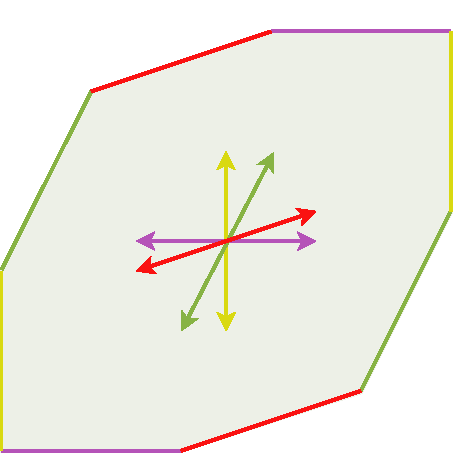
\includegraphics[trim={0 0 0 10},clip, width=0.6\linewidth]{img/chapter_2/zonotope_edges_parallel_generator.pdf}
      \end{minipage}
      \hfill
      \begin{minipage}{0.49\linewidth}
        \centering
        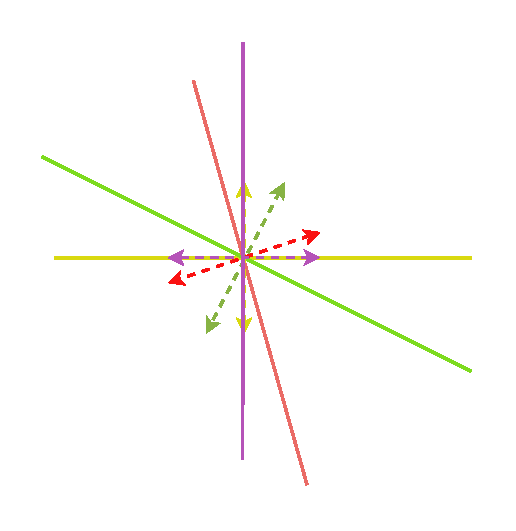
\includegraphics[trim={10 50 10 50},clip,width=0.8\linewidth]{img/chapter_2/central_arrangement.pdf}
      \end{minipage}
      \caption{Left: A zonotope with four generators. Right: The hyperplanes normal to each generator. This corresponds to its \emph{central hyperplane arrangement}.}
      \label{fig:zonotope_hyperplane_arrangement}
    \end{figure}
    
    \begin{figure}[!htb]
      \captionsetup{justification=centering}
      \centering
      
      \begin{minipage}{0.49\linewidth}
        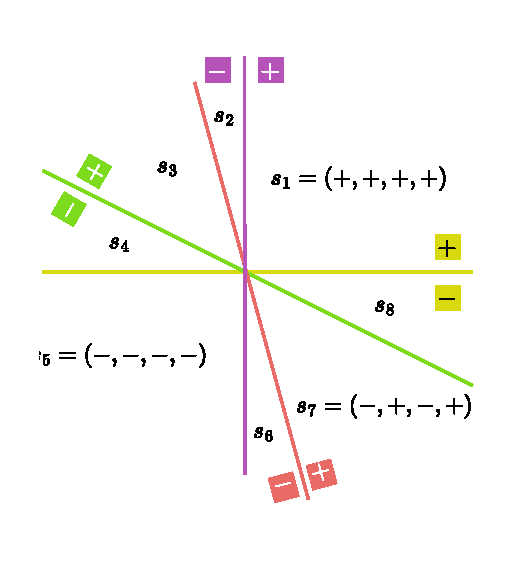
\includegraphics[trim={0 20 0 20},clip, width=0.9\linewidth]{img/chapter_2/sign_vectors_zonotope.pdf}
      \end{minipage}
      \hfill
      \begin{minipage}{0.49\linewidth}
        \hfill
        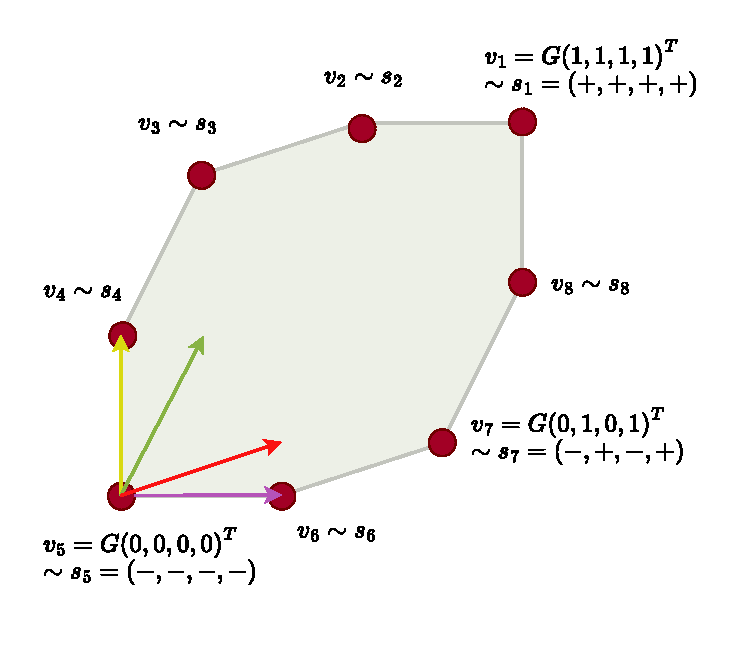
\includegraphics[trim={0 20 0 20},clip,width=1\linewidth]{img/chapter_2/zonotope_vertices_sign_vectors.pdf}
      \end{minipage}
      \caption{Let $G$ be the matrix with the yellow, purple, red, and green generators. In its central hyperplane arrangement, each region (or \emph{cell}) is represented by a sign vector $s_i$. Any $n$-dimensional space can be separated into exactly two half-spaces by a hyperplane. There are exactly as many cells as vertices in the underlying zonotope. Moreover, they are in one-to-one correspondence, as shown by the symbol $\sim$.}
      \label{fig:zonotope_hyperplane_arrangement2}
    \end{figure}

Due to the simplicity of working with sign vectors, there is a focus in computational geometry on creating algorithms dedicated to enumerating the cells of central hyperplane arrangements. Recent algorithms include those detailed in (\cite{radaNewAlgorithmEnumeration2018}), (\cite{guNonparametricMaximumLikelihood2020}), and (\cite{guCounterfactualIdentificationLatent2022}), whose practical performance surpasses the previous two. The latter algorithm will be described next.

\paragraph*{Gu et al.'s GRS algorithm (\cite{guCounterfactualIdentificationLatent2022}).}
This algorithm finds the cells of a central hyperplane arrangement iteratively over sub-dimensional arrangements. The main idea is to consider \emph{witness} points in each cell, whose signs correspond to a cell description, then remove one hyperplane from the arrangement and project all other hyperplanes onto the subspace it generates. The previous witness points are also projected onto this subspace, and they correspond to witness points of this sub-arrangement, up to duplication.
Figure \ref{fig:gu_et_al_algo} summarizes this process in two dimensions, where instead of projecting onto subspaces, the witness points are constructed iteratively.

\begin{figure}[!htb]
  \captionsetup{justification=centering}
  \centering
  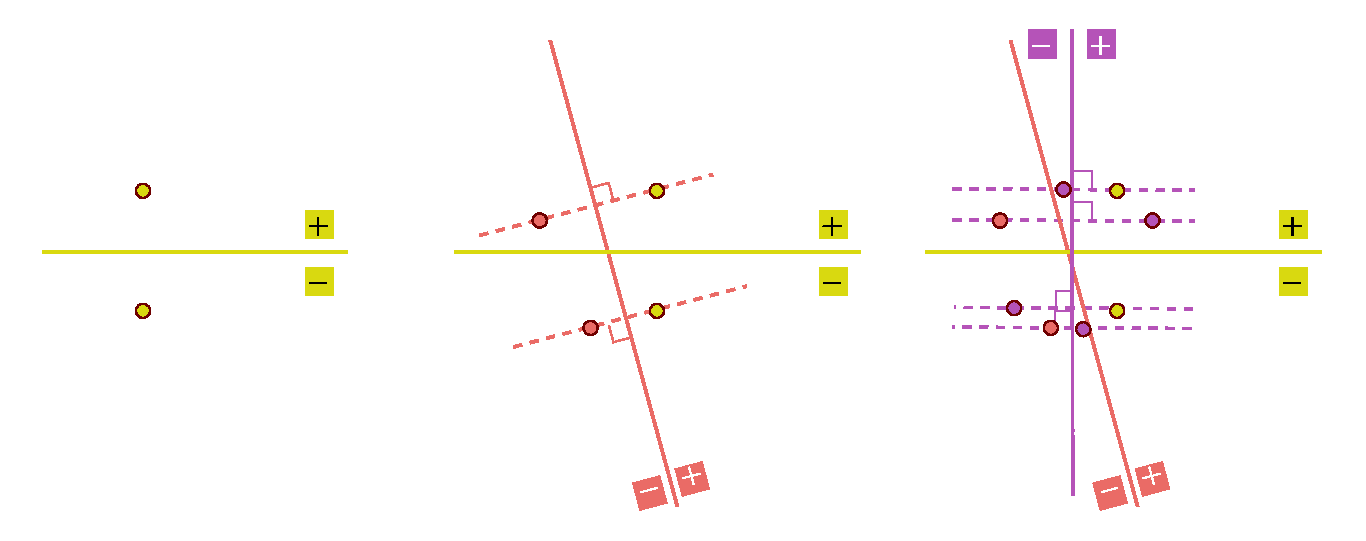
\includegraphics[trim={20 0 20 0},clip,width=1\linewidth]{img/chapter_2/gu_et_al_alg.pdf}
  \caption{Left: Two points are created on either side of the hyperplane. Middle: Another hyperplane is added, and the previously created points are copied to the other side of the new hyperplane. In (\cite{guCounterfactualIdentificationLatent2022}), the authors found a distance computation to ensure that the new points are in the closest region. Right: Repeat with another added hyperplane and remove duplicates, i.e., points with the same sign vector.}
  \label{fig:gu_et_al_algo}
\end{figure}

The two previous cell enumeration methods are interesting, given the correspondence between cells and vertices, but other algorithms exist to convert zonotope generators to a different representation, such as its bounding hyperplanes. However, since the focus here is on enumerating vertices, the conversion between bounding hyperplanes and vertices must be considered. Avis and Fukuda offer such a conversion algorithm in (\cite{avisPivotingAlgorithmConvex}) with a time complexity of $O(n_h n n_v)$, where $n$ is the dimension of $n_h$ hyperplanes, and $n_v$ is the number of vertices created by intersecting them. A method that uses bounding hyperplanes is detailed in the following paragraph.

\paragraph*{Gouttefarde and Krut's hyperplane shifting method (HS) (\cite{gouttefardeCharacterizationParallelManipulator2010a}).}
The number of bounding hyperplanes of a zonotope $\Zono(n,m)$ in general position is $f_{n-1}(\Zono) = 2\binom{m}{n-1}$, i.e., the $(n-1)$-dimensional faces of the $m$-cube project directly onto the zonotope's bounding hyperplanes. Since the position of each $(n-1)$-face in the $m$-cube is known, it remains to project the position and the $(n-1)$-space through the generator matrix and then compute the normal vectors. Using symmetry, the algorithm only needs to enumerate $\binom{m}{n-1}$ hyperplanes. Its time complexity is thus $O(\binom{m}{n-1})$ since all linear operations in the algorithm (computing normals, projecting, etc.) are necessarily bounded by $\binom{m}{n-1}$. This work utilizes the Python implementation package Pycapacity (\cite{skuricPycapacityRealtimeTaskspace2023}).

Table \ref{tab:theoretic_comparison_complexity} presents the time complexity of the three methods described above, compared to EdgeEnum.

\begin{table}[!ht]
    \centering
    \begin{tabular}{|c||c|c|c|c|}
    \hline
    Algorithm & \makecell{Pivot} & \makecell{HS} & \makecell{GRS} & \makecell{EdgeEnum} \\
    \hline
    \hline
    \makecell{Initial enumeration type} & Cell & Hyperplane & Cell & Edge \\ \hline
    \makecell{Time complexity} & $mf_0 \text{lp}(m,n$) & $\binom{m}{n-1}$ & $mf_0\text{mat}(m)$ & $nm^2f_1$ \\ \hline
    \makecell{Additional complexity \\ to convert to vertices} & $nmf_0$ & \makecell{$\binom{m}{n-1}nf_0$} & $nmf_0$ & $nmf_1$ \\ \hline
    \makecell{Total complexity \\ for $n$ fixed} & $m^{n+2.38}$ & $m^{2n-1}$ & $m^{n+1}$ & $m^{n+1}$ \\ \hline
    
    \end{tabular}
    \caption{Time complexity comparison between combinatorially equivalent enumeration algorithms when considering an $n$-dimensional zonotope with $m$ generators in general position. $f_0$ corresponds to its maximal number of vertices, and $f_1$ to its number of edges. Pivot denotes Avis and Fukuda's pivoting algorithm (\cite{avisPivotingAlgorithmConvex}), HS stands for Gouttefarde and Krut's hyperplane shifting method (\cite{gouttefardeCharacterizationParallelManipulator2010a}), and GRS is Gu et al.'s algorithm (\cite{guCounterfactualIdentificationLatent2022}). $\text{lp}(m,n)$ represents the time complexity to solve a linear program of $m$ equations with $n$ variables, and $\text{mat}(m)$ denotes the time cost to determine whether two vectors of length $m$ are identical. In (\cite{cohenSolvingLinearPrograms2020}), the authors created an algorithm that solves a linear program of $m$ equations and $n$ variables with the time complexity of matrix multiplication, approximately $m^{2.38}$. Using a programming language such as R or Python, $\text{mat}(m) = m$. In (\cite{avisPivotingAlgorithmConvex}), the created algorithm converts a set of $n_h$ hyperplanes to $f_0$ vertices with a time complexity of $O(n_h n f_0)$. The total complexity of HS is computed using Stirling's approximation of $\binom{m}{n}$ when $m$ gets large: $\binom{m}{n-1} \approx m^{n-1}/(n-1)! = O(m^{n-1})$ if $n$ is fixed.}
    \label{tab:theoretic_comparison_complexity}
\end{table}

The case of fixed $m$ and large $n$ is not of interest. If the number of generators $m$ is smaller than the dimension of the associated zonotope, enumerating the zonotope vertices necessarily requires enumerating \textbf{all} of the $m$-cube vertices (which amounts to $2^m$). Therefore, no algorithm can be more optimal than a naive algorithm that lists all the $m$-cube vertices.

However, a strong theoretical limitation arises when $m$ and $n$ grow at the same rate. For a preliminary analysis, note that when $n$ has approximately the same growth as $m$, $f_0(\Zono)$ is upper-bounded by $O(2^m)$, and $f_1(\Zono)$ is upper-bounded by $O(m2^{m-1})$ in the worst-case scenario (which occurs when $m=n$).
Thus, in this case, the algorithm with the best time complexity is that of (\cite{guCounterfactualIdentificationLatent2022}) (which grows as $O(m^2 2^m)$), while EdgeEnum lags behind, even preceded by a naive algorithm (of time complexity $O(m2^m)$), with a theoretical time complexity bounded by $O(m^4 2^{m-2})$. 

These results indicate that EdgeEnum theoretically performs similarly to the best state-of-the-art enumeration algorithm (\cite{guCounterfactualIdentificationLatent2022}) when there are many more generators than the ambient dimension of the produced zonotope. This scenario is relevant when considering a large number of muscles to produce the torque feasible set.

\section{Time benchmarks}
\label{time_benchmark}

Theoretical time complexity analysis is insufficient for a complete time study. A time benchmark must be performed on the different algorithms to evaluate the practical relevance of the edge-based vertex enumeration algorithm.
For instance, cell enumeration algorithms such as those in (\cite{radaNewAlgorithmEnumeration2018}) and \cite{guNonparametricMaximumLikelihood2020} have the same asymptotic bounds as in (\cite{avisPivotingAlgorithmConvex}) for hyperplane arrangements in dimensions greater than or equal to $3$, but they appear to exhibit faster computation times in practice (\cite{guCounterfactualIdentificationLatent2022}).

\subsection{Benchmark results}
\label{subsec:benchmark_results}

A computational time benchmark was performed to evaluate the relevance of a zonotope edge-based approach to vertex enumeration for faster computation. A Dell XPS15 laptop computer with a WSL2 and Ubuntu 22.01 operating system was used. This computer is equipped with 11th Gen Intel i9-11950H processors at 2.60GHz. Each core has two threads. The benchmark is implemented in Python 3.10 with the library \emph{numpy} 1.26.4 and default packages such as \emph{itertools} for rapidly generating cube vertices. The \emph{HS}, \emph{GRS}, and \emph{EdgeEnum} algorithms are implemented in Python, whereas \emph{Pivot} is implemented directly in C++ and uses the package \emph{libzonotope} for a Python interface. The edge-based algorithm requires a convex hull computation, which uses \emph{QuickHull}, available in Python through the library \emph{scipy}.


Table \ref{tab:benchmark_time} summarizes the means and standard deviations (in seconds) for each considered algorithm over 10 generator matrices $G\in\IRnm$, with values sampled from a uniform distribution between $-1$ and $1$.

\begin{table}[!ht]
    \centering
    \begin{tabular}{|c|c|c|c|c|}
    \hline
    $(n,m)$ & \makecell{Pivot} & \makecell{HS} & \makecell{GRS} & \makecell{EdgeEnum} \\
    \hline
    \hline

    % $(2, 10)$ & $<0.01$ & $<0.01$ & $<0.01$ & $<0.01$ \\
    % \hline
    $(2, 25)$ & $0.02 \pm 0.00$ & $\mathbf{<0.01}$ & $\mathbf{<0.01}$ & $0.02\pm 0.00$ \\
    \hline
    $(2, 50)$ & $0.08 \pm 0.00$ & $\mathbf{<0.01}$ & $\mathbf{<0.01}$ & $0.09\pm 0.00$ \\
    \hline
    \hline
    
    % $(3, 10)$ & $0.02\pm 0.00$ & $<0.01$ & $0.01\pm 0.00$ & $0.01 \pm 0.00$ \\
    % \hline
    $(3, 25)$ & $0.45\pm 0.01$ & $\mathbf{0.03\pm 0.00}$ & $0.04\pm 0.00$ & $0.14\pm 0.01$ \\
    \hline
    $(3, 50)$ & $4.25\pm 0.05$ & $\mathbf{0.14\pm 0.00}$ & $0.37\pm 0.02$ & $1.44\pm 0.03$ \\
    \hline
    \hline
    
    % $(4, 10)$ & $0.11\pm 0.00$ & $0.02\pm 0.00$ & $0.08\pm 0.01$ & $0.03\pm 0.01$ \\
    % \hline
    $(4, 15)$ & $0.66\pm 0.01$ & $\mathbf{0.08\pm 0.00}$ & $0.09 \pm 0.00$ & $0.14\pm 0.01$ \\
    \hline
    $(4, 20)$ & $2.41\pm 0.07$ & $\mathbf{0.21\pm 0.00}$ & $0.29\pm 0.01$ & $0.48\pm 0.02$ \\
    \hline
    \hline

    % $(5, 10)$ & $0.34\pm 0.02$ & $0.09\pm 0.00$ & $0.30\pm 0.00$ & $0.10\pm 0.00$ \\
    % \hline
    $(5, 15)$ & $3.60\pm 0.08$ & $0.80\pm 0.01$ & $\mathbf{0.42\pm 0.01}$ & $0.97\pm 0.01$ \\
    \hline
    $(5, 20)$ & $17.99\pm 0.14$ & $4.25\pm 0.06$ & $\mathbf{2.80\pm 0.11}$ & $6.55\pm 0.29$ \\
    \hline
    \hline

    $(6, 10)$ & $0.73\pm 0.02$ & $0.58\pm 0.05$ & $\mathbf{0.10\pm 0.00}$ & $0.43\pm 0.01$ \\
    \hline
    $(6, 11)$ & $1.48\pm 0.05$ & $1.39\pm 0.12$ & $\mathbf{0.19\pm 0.01}$ & $0.92\pm 0.01$ \\
    \hline
    $(6, 12)$ & $2.73\pm 0.07$ & $2.86\pm 0.22$ & $\mathbf{0.33\pm 0.02}$ & $1.80\pm 0.05$ \\
    \hline
    \end{tabular}
    \caption{Mean and standard deviation of computation time (in seconds) for $10$ randomly generated zonotopes using different zonotope enumeration algorithms. All generators are in general position, and all algorithms returned the expected number of vertices, $f_0$. The conversion time from a specific representation to vertices is included for each algorithm.}
    \label{tab:benchmark_time}
\end{table}

The hyperplane shifting algorithm (HS) is the fastest in almost all cases for $n\leq 4$, even though it theoretically has the worst time complexity of the presented algorithms. However, as the dimension $n$ increases, its complexity grows combinatorially, which could explain why GRS is the fastest from dimension 5 onward. While EdgeEnum exhibits equivalent time complexity than GRS, the difference observed probably result from the asymptotic growth on the number of $k$-faces  in Lemma \ref{th:big_O_nb_k_faces}: while it states that vertices or edges number has an asymptotic growth in $O(m^{n-1})$, this does not mean that the number of edges is similar to the number of vertices. It is much higher, and is reflected in the time computation benchmark. 

\subsection{Parallelization of EdgeEnum}

To improve the time performance of EdgeEnum, \emph{parallelization} could be employed. This refers to distributing parts of an algorithm across multiple processors. Not all algorithms can be parallelized, but for those that can, computation times can be drastically improved.

In EdgeEnum, one part can be distributed: the inner loop in which the convex hull of each group of edges is computed. The new edges gathered after an iteration of this loop do not influence the gathering of other iterations, making it parallelizable. For instance, using the same computational setup as described previously, Table \ref{tab:parallelism_time_benchmark} summarizes the performance of EdgeEnum using either a single processor or two.

\begin{table}[!ht]
    \centering
    \begin{tabular}{|c|c|c|c|c|}
    \hline
    $(n,m)$ & \makecell{EdgeEnum} & \makecell{EdgeEnum Parallel} \\
    \hline
    \hline
    
    $(6, 10)$ & $0.43\pm 0.01$ & $0.14\pm 0.01$ \\ 
    \hline
    $(6, 11)$ & $0.92\pm 0.01$ & $0.28\pm 0.02$ \\
    \hline
    $(6, 12)$ & $1.80\pm 0.05$ & $0.54\pm 0.03$ \\
    \hline
    \end{tabular}
    \caption{Mean and standard deviation of computation time (in seconds) for $10$ randomly generated generator matrices $G\in\IRnm$ per tuple $(n,m)$. EdgeEnum is parallelized across two processors using the Python package \emph{multiprocessing}.}
    \label{tab:parallelism_time_benchmark}
\end{table}

It is noteworthy that the parallelization only appears to have a non-negligible effect for $n\geq 6$. For lower values of $n$, parallelization results in worse computation times due to the overhead required to copy and transfer data between processors. The parallelized version is not compared with other algorithms here, as they are implemented in a non-parallelized manner.

\subsection{Conclusion on practical time computation}
In conclusion, computing the vertices of a zonotope $\Zono(n,m)$ requires significant computation time, even though the edge-based approach demonstrates time-theoretic efficiency. This is due to the combinatorial explosion in the number of zonotope vertices as the number of generators increases. When modeling force or torque feasible sets using a musculoskeletal model, especially in an optimization context where the goal is to find a set of parameters that reproduce \emph{in silico} and \emph{in vivo} force feasible sets (cf. Chapters \ref{chapter:4} and \ref{chapter:5}), a large number of these sets must be computed. As the number of muscles considered increases, the search space expands, necessitating the evaluation of more solutions. A computation time of $\leq 0.2$ seconds for zonotope vertices leads to hours of optimization when considering a reasonably sufficient number of muscles ($\geq 20$).

Because computation time is a major obstacle, approximations of the vertex set of a zonotope will be explored. Their relevance will be assessed in terms of both computation time and the shape they produce.

\section{Approximation of the vertex set}
\label{sec:approximation_of_vertices_zonotope}
While the methods described previously provide the \emph{exact} vertices of a zonotope, the number of vertices to enumerate is a computational bottleneck for all previously cited algorithm: there are too many to store. This often occurs when the number of generators is large, regardless of the dimension $n$. Thus, it is desirable to reduce computation time through approximations.

Approximating the surface of a zonotope can be done in multiple ways, including bounding boxes or various ellipsoid approximations (\cite{cernyGoffinAlgorithmZonotopes2012}; \cite{gasmannScalableZonotopeEllipsoidConversions2020}; \cite{kousikEllipsotopesCombiningEllipsoids2021}; \cite{henkLownerJohnEllipsoids2012}). However, their main drawback is that they do not necessarily preserve the shape of the zonotope. Generally, the quality of the approximation is related to the computation time.

This work focuses on preserving the shape of a zonotope by approximating its vertex set. This can be achieved in two ways: either by computing a subset of vertices that sufficiently expresses the zonotope shape or by finding points close to each zonotope vertex, up to some tolerance. These two approaches are represented by the following algorithms:

\paragraph*{Stinson et al. randomized vertex enumeration (\cite{stinsonRandomizedAlgorithmEnumerating2016}).}
For a zonotope $\Zono(G)$ with $G\in \IRnm$, this algorithm samples vectors in the zonotope space $\IRn$ using a standard Gaussian distribution in $\IRm$. These vectors are then projected onto $\IRm$ via the map $\mathbf{x}\mapsto \text{sign}(G^T\mathbf{x})$, where $\text{sign}$ assigns $-1$ if its input is negative and $1$ otherwise. The resulting vector in $\IRm$ corresponds to a vertex of the $m$-cube. Stinson et al. showed that a vertex created in this way maps to a zonotope vertex with probability $1$. This approach is inherently fast, as it only requires sampling a chosen number of vectors in $\IRn$. However, a significant caveat arises if the zonotope generators have mutually close angles, as shown in Figure \ref{fig:stinson_fail}. In this case, many randomly chosen vectors may map to the same zonotope vertex and rarely to others. To mitigate this, the sampling size must be increased.

\begin{figure}[!htb]
  \captionsetup{justification=centering}
  \centering
  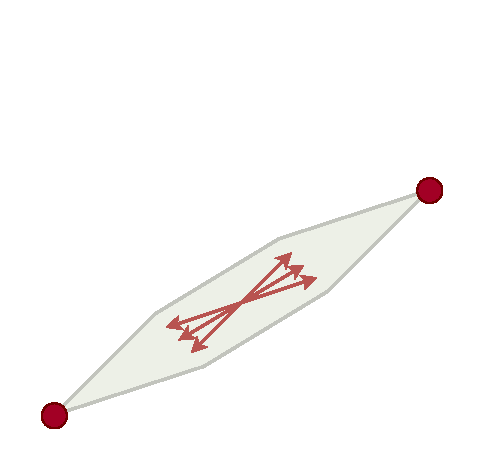
\includegraphics[trim={0 0 0 80},clip, width=0.5\linewidth]{img/chapter_2/stinson_algo_fail.pdf}
  
  \caption{(\cite{stinsonRandomizedAlgorithmEnumerating2016})'s randomized vertex enumeration algorithm. This is an example where the generators have mutually close angles. In this case, the chosen random vectors have a high probability of corresponding to the same zonotope vertex (in red). The sampling size must be increased to avoid this effect.}
  \label{fig:stinson_fail}
\end{figure}

\paragraph*{Skuric et al.'s iterative convex hull method (ICH) (\cite{skuricOnLineFeasibleWrench2022}).}
Recently, a new approximation method for polytope surfaces was proposed in (\cite{skuricOnLineFeasibleWrench2022}). Figure \ref{fig:ich_method} summarizes this method. For a zonotope $\Zono(n,m)$ in $\IRn$, the algorithm begins by selecting $n$ direction vectors in $\IRn$ and then identifies the closest vertices to these directions using a linear program. Iteratively, by selecting new directions based on the normals of the polytope constructed from the convex hull of the found vertices, this algorithm enumerates vertices until a specified tolerance representing how close vertices are from the created directions.
A Python implementation is available and described in (\cite{skuricPycapacityRealtimeTaskspace2023}).

% \begin{figure}[!htb]
%   \captionsetup{justification=centering}
%   \centering
%   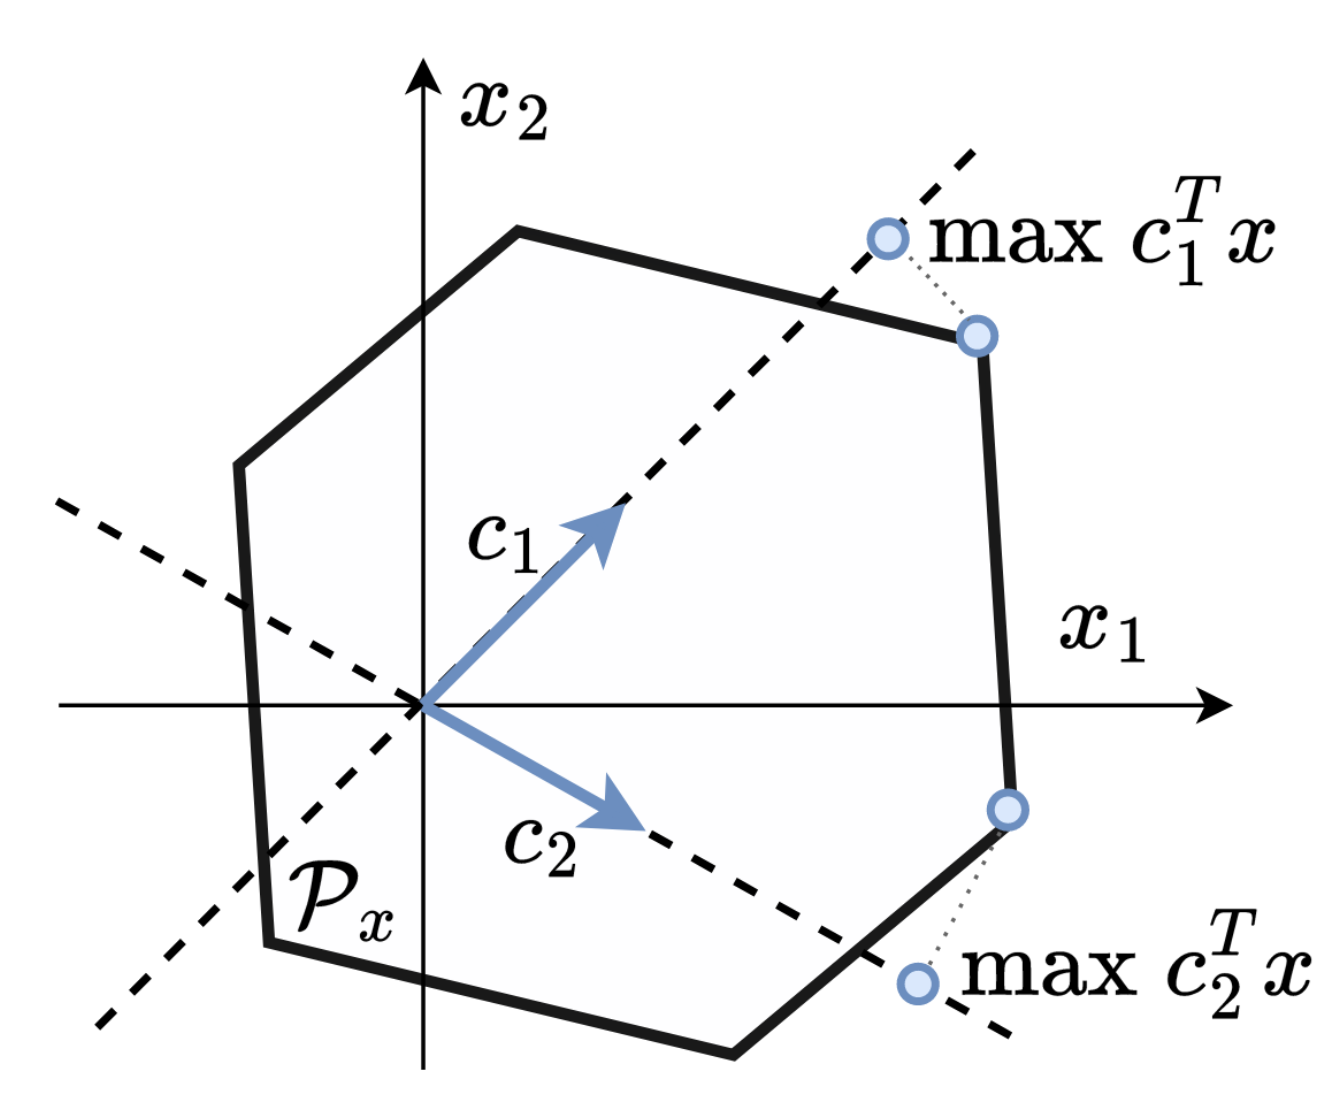
\includegraphics[trim={0 0 0 0},clip, width=0.4\linewidth]{img/chapter_2/ich_alg0.png}
  
%   \caption{Illustration of the Iterative Convex Hull algorithm. Image from (\cite{skuricCoupledViewPhysical}).}
%   \label{fig:ich_method}
% \end{figure}

\begin{figure}[!htb]
    \captionsetup{justification=centering}
    % \begin{minipage}{1\linewidth}
    %     \centering
    %     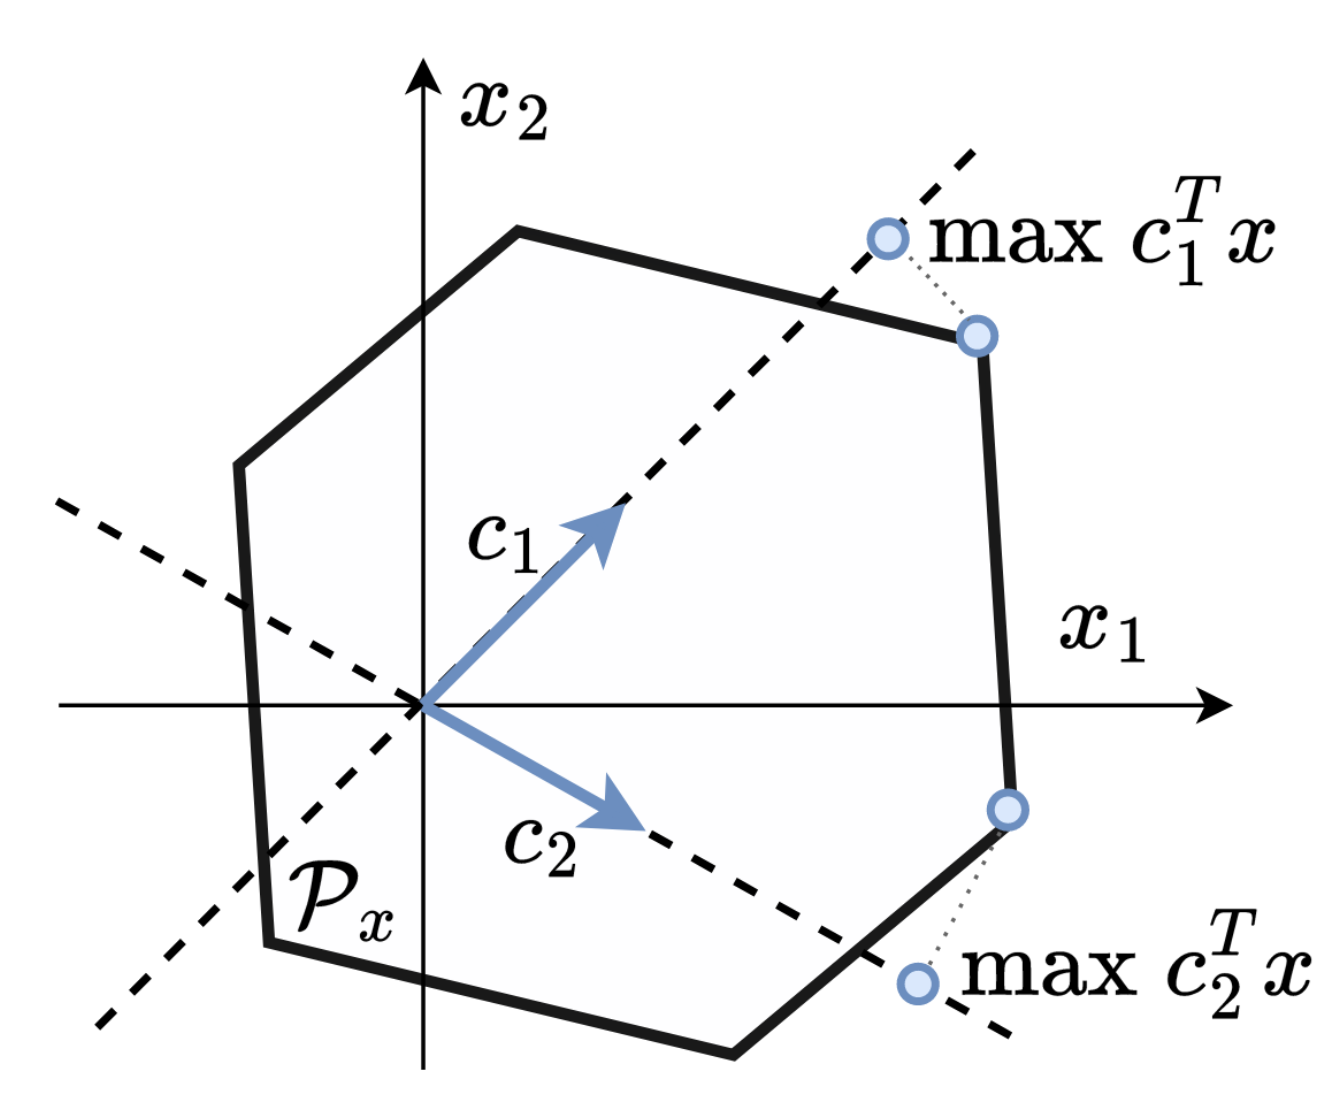
\includegraphics[trim={0 0 0 0},clip, width=0.4\linewidth]{img/chapter_2/ich_alg0.png}
    %     \caption{First step .}
    % \end{minipage}
        \centering
        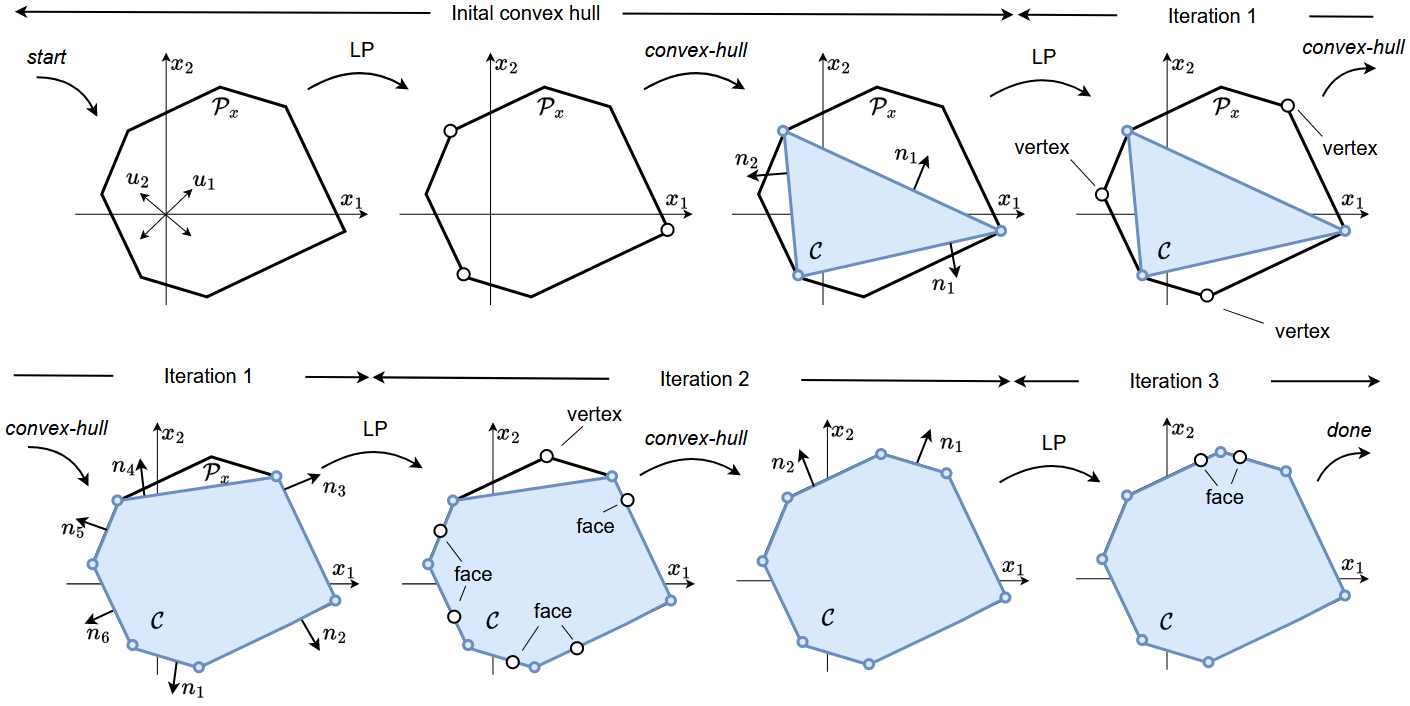
\includegraphics[trim={0 0 0 0},clip, width=1\linewidth]{img/chapter_2/ich_alg.png}
    % \hfill
    % \begin{minipage}{1\linewidth}
    %     \centering
    %     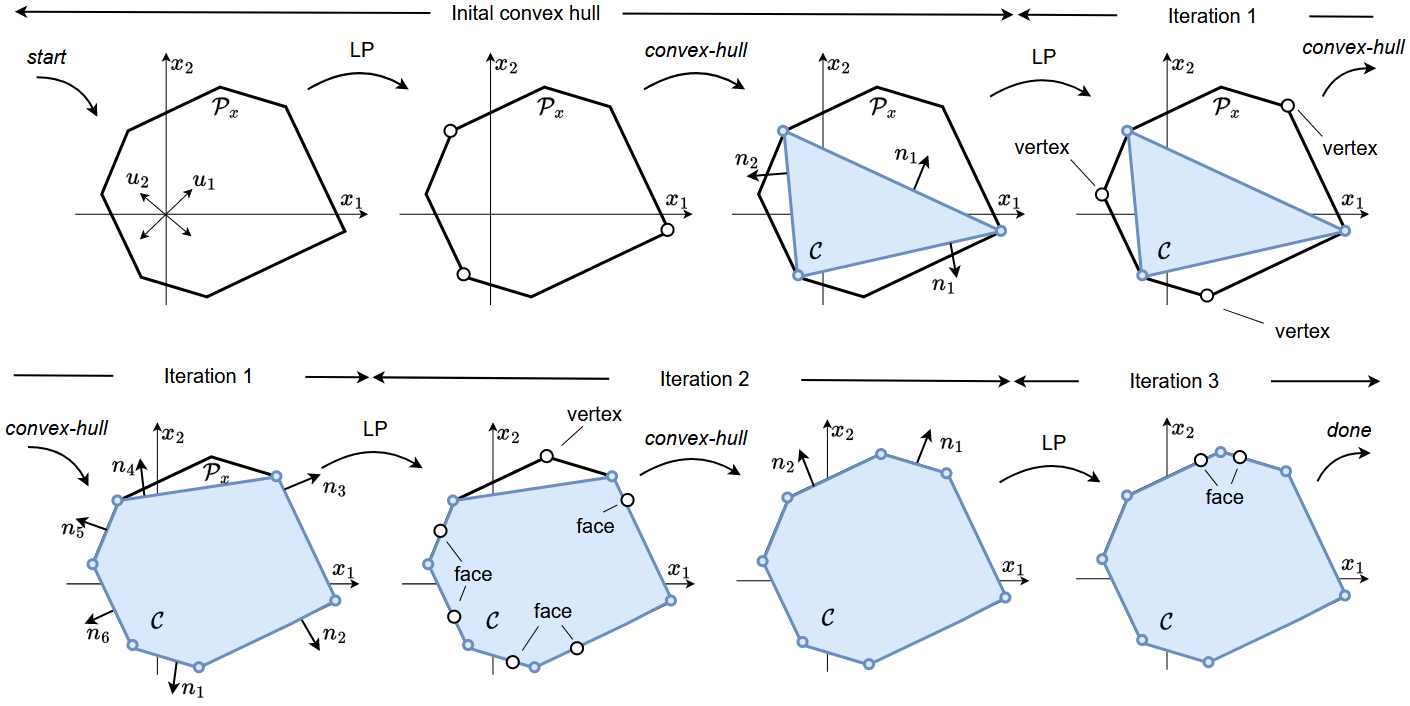
\includegraphics[trim={0 0 0 0},clip, width=1\linewidth]{img/chapter_2/ich_alg.png}
    % \end{minipage}
    \caption{Illustration of the Iterative Convex Hull algorithm. Image from (\cite{skuricCoupledViewPhysical}).}
    \label{fig:ich_method}
\end{figure}

To compare the quality of the vertices produced by each of these algorithms, a suitable metric must be defined. While the Hausdorff distance, a computable distance between sets of points involving the Euclidean distance from every point of one set to every point of another, exists, it is not necessarily a relevant metric in this context. Skuric et al.'s method returns a considerable number of points close to the surface of the zonotope, far exceeding the expected number of vertices. Since the primary interest lies in the global shape of the zonotope, comparing the relative distances of the returned points and the exact vertices would not provide strong information on whether the zonotope's surface is well-approximated. Instead, this work uses the \emph{Jaccard index}, also called the Jaccard similarity coefficient. It is defined for any two sets $A$ and $B$ as
$$J(A, B) = \frac{\text{Vol}(A\cap B)}{\text{Vol}(A\cup B)}$$ where $\text{Vol}$ denotes the volume. 

The Jaccard index, which measures the similarity between two sets, attains a value of 1 when the sets are identical, indicating perfect overlap. For both algorithms presented, the returned points lie \emph{on} the surface of the given zonotope, so the intersection and union are easily computed.

Tables \ref{tab:approx_vertex_set_stinson} and \ref{tab:approx_vertex_set_ich} summarize the computation times for both algorithms for $4$-dimensional zonotopes with $m=15$ or $m=20$ generators, respectively. Table \ref{tab:approx_vertex_set_stinson} shows the results for the randomized enumeration algorithm, and Table \ref{tab:approx_vertex_set_ich} shows the results for ICH algorithm. All computations were performed using the same setup as the previous time benchmark in Subsection \ref{subsec:benchmark_results}.

\begin{table}[!ht]
    \centering
    \begin{tabular}{|c|c|c|c|c|}
    \hline
    $(n,m)$ & \makecell{Number of \\ samples} & \makecell{Computation \\ time} & \makecell{Number found points \\ / exact number of vertices} & \makecell{Jaccard \\ index} \\
    \hline
    \hline

    % $(2, 10)$ & $<0.01$ & $<0.01$ & $<0.01$ & $<0.01$ \\
    % \hline
    \multirow{ 4}{*}{$(4,15)$} & $10$ & $<0.01$ & $0.41\pm 0.03$ & $0.98\pm 0.01$  \\
    \cline{2-5}
     & $100$ & $<0.01$ & $0.67\pm 0.05$ & $\mathbf{1.00\pm 0.00}$  \\
     \cline{2-5}
     & $1000$ & $0.05\pm 0.00$ & $0.83\pm 0.02$ & $\mathbf{1.00\pm 0.00}$ \\
    \cline{2-5}
     & $10000$ & $0.30\pm 0.01$ & $0.93\pm 0.01$ & $\mathbf{1.00\pm 0.00}$ \\
    % \cline{2-4}
    \hline
    \multirow{ 4}{*}{$(4,20)$} & $10$ & $<0.01$ & $0.28\pm 0.01$ & $0.97\pm 0.00$ \\
    \cline{2-5}
     & $100$ & $0.02\pm 0.00$ & $0.56\pm 0.03$ & $\mathbf{1.00\pm 0.00}$ \\
    \cline{2-5}
     & $1000$ & $0.08\pm 0.00$ & $0.78\pm 0.03$ & $\mathbf{1.00\pm 0.00}$ \\
    \cline{2-5}
     & $10000$ & $0.39\pm 0.02$ & $0.89\pm 0.01$ & $\mathbf{1.00\pm 0.00}$ \\
    \hline
    \end{tabular}
    \caption{Performance of (\cite{stinsonRandomizedAlgorithmEnumerating2016})'s randomized algorithm. For each row, $10$ randomly generated $4$-dimensional zonotopes with $m$ generators are computed. The `Number of Samples' column indicates the number of vertices randomly drawn at each iteration. Computation times are in seconds.}
    \label{tab:approx_vertex_set_stinson}
\end{table}

\begin{table}[!ht]
    \centering
    \begin{tabular}{|c|c|c|c|c|}
    \hline
    $(n,m)$ & Tolerance & \makecell{Computation \\ time} & \makecell{Number found points \\ / exact number of vertices} & \makecell{Jaccard \\ index} \\
    \hline
    \hline

    % $(2, 10)$ & $<0.01$ & $<0.01$ & $<0.01$ & $<0.01$ \\
    % \hline
    \multirow{ 4}{*}{$(4,15)$} & $1$ & $0.03\pm 0.01$ & $0.03\pm 0.01$ & $0.56\pm 0.05$  \\
    \cline{2-5}
    & $0.1$ & $0.29\pm 0.02$ & $0.72\pm 0.10$ & $0.98\pm 0.00$ \\
    \cline{2-5}
    & $0.01$ & $0.39\pm 0.01$ & $1.94\pm 0
    .6$ & $\mathbf{1.00\pm 0.00}$\\
    \cline{2-5}
    & $0.001$ & $0.39\pm 0.02$ & $2.12\pm 0.04$ & $\mathbf{1.00\pm 0.00}$ \\
    \hline
    \multirow{ 4}{*}{$(4,20)$}& $1$ & $0.06\pm 0.01$ & $0.03\pm 0.01$ & $0.68\pm 0.05$ \\
    \cline{2-5}
    & $0.1$ & $0.54\pm 0.03$ & $0.61\pm 0.05$ & $0.99\pm 0.00$ \\
    \cline{2-5}
    & $0.01$ & $0.64\pm 0.04$ & $1.36\pm 0.07$ & $\mathbf{1.00\pm 0.00}$ \\
    \cline{2-5}
    & $0.001$ & $0.62\pm 0.04$ & $1.37\pm 0.07$ & $\mathbf{1.00\pm 0.00}$ \\
    \hline
    \end{tabular}
    \caption{Performance of (\cite{skuricOnLineFeasibleWrench2022})'s ICH algorithm. For each row, $10$ randomly generated $4$-dimensional zonotopes with $m$ generators are computed. The "Tolerance" column indicates how close a computed point should be to the zonotope surface. Computation times are in seconds.}
    \label{tab:approx_vertex_set_ich}
\end{table}

These tables confirm that both algorithms can produce a set of points that yield a shape similar to that of a given zonotope. Stinson et al.'s algorithm produces such a set very quickly compared to exact algorithms, with a number of required points much smaller than the exact amount. However, Škuric et al.'s method requires setting a low tolerance to ensure that the points it produces are close to the zonotope surface, leading to longer computation times associated with a larger number of generated points. 

While the results concerning exact and approximation algorithms relate to the surface description of a zonotope, the problems are fundamentally different. This section demonstrated that in the context of describing the shape of the torque feasible set, an exact enumeration algorithm should \textbf{not} be used when considering a large number of muscles. However, working with exact algorithms provided insights into the geometric processes that occur when describing the projection of a tension feasible set modeled as an orthotope. This understanding is key to generalizing the projection process for any convex shape of $\mathcal{T}$, which is the focus of Chapter \ref{chapter:3}.

\section{Conclusion}
\label{conclusion_zonotope_enum_algorithm}
This chapter focused on explicitly computing the torque feasible set 
\begin{align*}
    \left\{\tau \in \IR^n \mid \exists \mathbf{t}\in\mathcal{T}, \quad \tau = -L^T\mathbf{t} - \mathbf{G}\right\}
\end{align*}
assuming that $\mathcal{T}$ is an orthotope, and without loss of generality, an $m$-dimensional cube. The resulting set is a zonotope, which can be described through various representations, including a set of vertices. However, in this case, the torque feasible set is associated with the matrix $-L^T$, which does not directly reveal the global shape of its associated zonotope. 

This chapter proposed an efficient algorithm, called EdgeEnum, to compute the exact vertices of a zonotope based on its edge enumeration. Its time and space complexity were compared theoretically with those of several state-of-the-art zonotope vertex enumeration algorithms, demonstrating that EdgeEnum is a theoretically performant algorithm for worst-case scenarios, i.e., when the number of columns of $-L^T$ is large compared to its number of rows ($n\ll m$).

However, in practice, the algorithm may not be performant due to the unavoidable combinatorial number of edges to enumerate. A time benchmark was performed to highlight this issue. The following paragraphs summarize the benefits and limitations of using an edge-based algorithm.

\subsection*{Strengths of EdgeEnum}

EdgeEnum has several advantages, from its creation process to its implementation.

\paragraph*{Ease of implementation.} EdgeEnum is straightforward to implement. While a recursive version is possible (and implemented in its associated Python package), this chapter presented an implementation based on an iterative construction of the edges of an $m$-cube to emphasize readability and geometric intuition. The only requirement for implementation in any language is the availability of a convex hull operation, which is already natively implemented or available through dedicated libraries in common scientific programming languages such as R, MATLAB, Python, and Julia.

\paragraph*{Parallelism.} A significant advantage of EdgeEnum compared to recent developments is its suitability for parallelization, unlike recent developments such as in (\cite{guCounterfactualIdentificationLatent2022}). This parallelization occurs during the grouping process, in which all current edges during an iteration are separated into groups according to their directions. Applying the convex hull to one group of edges does not require the resulting convex hull of another group. The Python implementation offers both parallel and non-parallel versions of EdgeEnum.

\paragraph*{Theoretical efficiency when $n$ is fixed.} Theorems \ref{th:time_complexity_n_fixed} and \ref{th:space_complexity_n_fixed} showed that the time and space complexity of the algorithm are polynomially bounded in the input and output sizes. This is fundamental, as it qualifies EdgeEnum as an efficient algorithm in terms of both time and space. 

% \paragraph*{Faster than state-of-the-art Algorithms for Large $m$ and $n>6$.} While related to the theoretical notion of efficiency, the numerical time benchmarks show that in practice, EdgeEnum is indeed faster than state-of-the-art algorithms when dealing with a zonotope with a generator matrix in $\IRnm$. Note that for $n=2$, the algorithm can never be better than that of Gu et al. \cite{guCounterfactualIdentificationLatent2022}, as their algorithm reaches near-optimality in this specific case.

\paragraph*{Handling degeneracy.} Degeneracy of a zonotope describes whether its generators are in general position. If they are, the zonotope is not degenerate. The only condition to handle degeneracy is the ability of the convex hull operation to return multiple points that are located at the same position. In this case, the convex hull time complexity is not $O(n\log h)$, where $n$ is the number of points, and $h$ is the number of points on the convex hull. Instead, it is $O(n\log n)$ on average, using an algorithm like \emph{QuickHull} (\cite{barberQuickhullAlgorithmConvex1996}). When applying this new bound to the computed theoretical complexities, the result does not change. However, the computed complexities become \emph{average} bounds, not worst-case bounds. 

The following paragraphs describe several drawbacks of EdgeEnum.

\subsection*{Limits}
This chapter identified three types of limitations related to theoretical algorithmic results, extension of the method to polytopes, and the thesis's goal of understanding the zonotope surface.

\paragraph*{Non-compactness.} An algorithm is \emph{compact} if its space complexity is polynomially bounded by the input size alone (\cite{fukudaZonotopeConstructionMinkowski2004a}).
While the new approach has polynomial time and space complexity for fixed $n$, it requires storing all edges found in each iteration. Therefore, the algorithm does not have the property of \emph{compactness} as its space complexity is not polynomially bounded by the input size alone (\cite{fukudaZonotopeConstructionMinkowski2004a}). The input size is determined by the generator matrix, which has size $nm$. Even for fixed $n$, the space complexity is $O(m^{n+2})$ and is not bounded by any polynomial $(nm)^{\alpha}$, where $\alpha$ is a positive real number. In other words, the algorithm cannot stream edges once they are found, since an edge may be rejected in a subsequent iteration.

As explained in (\cite{ferrezSolvingFixedRank2005a}), the algorithm falls into the category of \emph{incremental} strategies. This means that the edge enumeration problem is solved inductively by maintaining a list of edges at a certain state. The memory requirement is a critical disadvantage of this kind of approach. Thus, the time efficiency of the algorithm is counteracted by its space requirements.

\paragraph*{Approximation algorithms are better suited for fast zonotope surface description.} 
Even though EdgeEnum remains relevant for some practical problems (\cite{guCounterfactualIdentificationLatent2022}; \cite{fukudaZonotopeConstructionMinkowski2004a}; \cite{guibasZonotopesBoundingVolumes}), it may not be the most suitable choice for describing a zonotope surface. Approximation algorithms can achieve compelling results with significantly faster computation times by identifying a limited number of points on the surface. The convex hull of these points closely approximates the desired zonotope (in terms of volume), as demonstrated in Section \ref{sec:approximation_of_vertices_zonotope}.

Consequently, for the remainder of this thesis, all vertex computations of force feasible sets represented as polytopes will employ an approximation approach. Since Chapter \ref{chapter:4} involves computing a large number of force polytopes to determine the parameters of a musculoskeletal model from \emph{in silico} force polytopes, the Iterative Convex Hull method (\cite{skuricOnLineFeasibleWrench2022}) will be used for all polytope computations. The chosen tolerance will vary depending on the context.

\paragraph*{EdgeEnum does not (always) extend to the vertex enumeration of zonotope sections.} While this chapter presented results concerning the torque feasible set, our thesis focuses on force feasible sets, including those modeled as polytope, i.e., a section of a zonotope. If $p$, the dimension of this section, equals $n-1$, then it is possible to construct some vertices of the polytope resulting from this section (cf. Figure \ref{fig:zonotope_section_2D_example}). If the affine subspace sectioning the zonotope is in general position (i.e., it does not cross any vertices of the zonotope), then it is even possible to enumerate all of its vertices. However, in this context, the force feasible set is usually described in 3D, the torque space in 7D, and the tension space in $mD$ for $m\geq 7$, so it is not possible to return all vertices. This is mainly because the polytope vertices are produced by intersecting this affine space with higher-dimensional faces of the zonotope, not necessarily \emph{only} with edges.

\begin{figure}[!htb]
  \captionsetup{justification=centering}
  \centering
  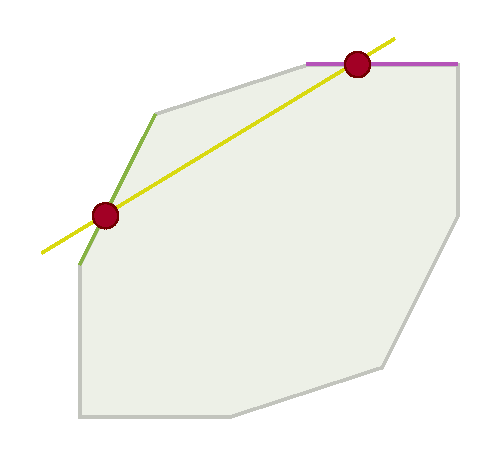
\includegraphics[trim={0 0 0 0},clip, width=0.4\linewidth]{img/chapter_2/polytope_section_zono.pdf}
  \caption{An affine subspace $L$ of dimension $1$ that does not intersect any zonotope vertices is shown in yellow. In this case, because $1 = n-1$, where $n=2$ is the dimension of the zonotope, it is possible to construct the vertices of this zonotope section by intersecting $L$ with the edges it crosses.}
  \label{fig:zonotope_section_2D_example}
\end{figure}

\subsection*{On the cubical representation of the tension feasible set}
The novel algorithm presented in this chapter is theoretically relevant to the vertex enumeration subfield of computational geometry. It sheds new light on enumeration techniques. To the best of our knowledge, most enumeration algorithms consider cube vertices, hyperplanes, and sign vectors, but rarely edges. This may be because the number of cube edges is much larger than the number of cube vertices.

In practice, the number of zonotope vertices grows combinatorially with its number of generators, making \emph{any} enumeration algorithm inefficient with regard to computation time. Section \ref{sec:approximation_of_vertices_zonotope} considered approximations of the zonotope surface to further decrease computation time and reduce the number of points required to describe the zonotope surface. These approximations are relevant in the context of this thesis. 

To reconstruct a musculoskeletal model whose torque feasible sets fit given maximal torque capacities in various postures, it must be possible to generate \emph{in silico} a large number of torque feasible sets and compare them.

However, whether approximations or exact algorithms are used, it was hypothesized that the tension feasible set is shaped as a cube. Biomechanically, this means that all muscles can produce their maximum tensions simultaneously. The next chapter will consider other shapes and their associated biomechanical assumptions to focus on their produced force feasible set shape. The creation process of EdgeEnum is a first step in this direction. This chapter described the global shape of the torque feasible set by navigating between the tension feasible set and its projection onto the torque space. More generally, the shape of the tension feasible set and its projection (followed or not by an intersection) are strongly linked. They are even \emph{inextricable}, and the main results of the next chapter argue that the shape of the tension feasible set does not strictly matter when a large number of muscles is considered. Surprisingly, these results will lead to a new characterization of force feasible sets and a deeper understanding of muscle tension interactions.
